\chapter{Inecuaciones y sistemas}

\begin{tikzpicture}
	\fill [left color=red!50, right color=teal!50] (0,0) rectangle (6.5,.2);
	\fill [left color=teal!50, right color=blue!50] (6.5,0) rectangle (11.5,.2);
	\end{tikzpicture}


\vspace{5mm}
\begin{adjustwidth}{40pt}{40pt}
\begin{cuadro-gris}

	\begin{multicols}{2}
	
	$\triangleright \quad$  Inecuaciones con una incógnita: 
	
	$\qquad $--- lineales  
	
	$\qquad $--- no lineales.	
	
	$\triangleright \quad$  Sistemas de inecuaciones con una incógnita.
	
	$\triangleright \quad$ Inecuaciones y sistemas lineales con dos incógnitas.
	\end{multicols}
	
\end{cuadro-gris}
\end{adjustwidth}

\vspace{1cm}
\begin{definition}
.	Una inecuación es una desigualdad algebraica en la que sus dos miembros aparecen ligados por uno de estos signos $\ <\, , \ \ >\, , \ \ \leqslant \, \ \ \geqslant$. 

\vspace{2mm} La solución de una inecuación es el conjunto de valores de la variable que verifica la inecuacíón, serán intervalos de la recta real.
\end{definition}
\vspace{5mm}

\begin{myexampleblock}{Historia de las inecuaciones}

\vspace{2mm} No se sabe exactamente el origen de las inecuaciones pero se cree que se originaron poco después de las ecuaciones (1700aC. – 1700dC.) debido al surgimiento de un problema en el cual la respuesta podía contener un grupo de números.

\vspace{2mm} Una inecuación es una expresión matemática la cual se caracteriza por tener los signos de desigualdad.

\vspace{2mm} La notación $\ a < b \ $ significa que $a$ es menor que $b$ y la notación $\ a > b \ $ quiere decir que $a$ es mayor que $b$. Estas relaciones son conocidas con el nombre de desigualdades estrictas, contrastando con $ \ a \leqslant b\ $ ($a$ es menor o igual que $b$  y $\ a \geqslant b\ $ ($a$ es mayor o igual que $b$).

\vspace{2mm} La notación $\ a >> bº $ quiere decir que $a$ ``es mucho mayor'' que $b$. 
	
\end{myexampleblock}


\vspace{5mm}
\begin{theorem}
.	Hay que tener en cuenta que:

\begin{itemize}
\item Si a los dos miembros de una inecuación se les suma o se les resta un mismo número, la inecuación resultante es equivalente a la dada.
\item Si a los dos miembros de una inecuación se les multiplica o divide por un mismo número positivo, la inecuación resultante es equivalente a la dada.
\item Si a los dos miembros de una inecuación se les multiplica o divide por un mismo número negativo, la inecuación resultante cambia de sentido y es equivalente a la dada.
\end{itemize}
\end{theorem}

\vspace{5mm}

\begin{multicols}{2}
	\begin{destacado}
	\vspace{2mm}$2<5 \ \to \ 2+7<5+7\Rightarrow 9<12$

	$2<5 \ \to \ 2\cdot 3 < 5\cdot 3 \Rightarrow 6<15$

	$2<5 \ \to \ 2\cdot (-4) < 5\cdot (-4) \Rightarrow -8 \boldsymbol >-20$

	\vspace{2mm}Al multiplicar (dividir) toda una una inecuación por un número negativo, \emph{el sentido de la desigualdad \textbf{cambia}}: $<$ se convierte en $>$, $\ \leqslant$ se convierte en $\geqslant$, $\ >$ se convierte en $<$ y $\ \geqslant$ en $\leqslant$.
	\vspace{2mm}
	\end{destacado}

	\begin{figure}[H]
		\centering
		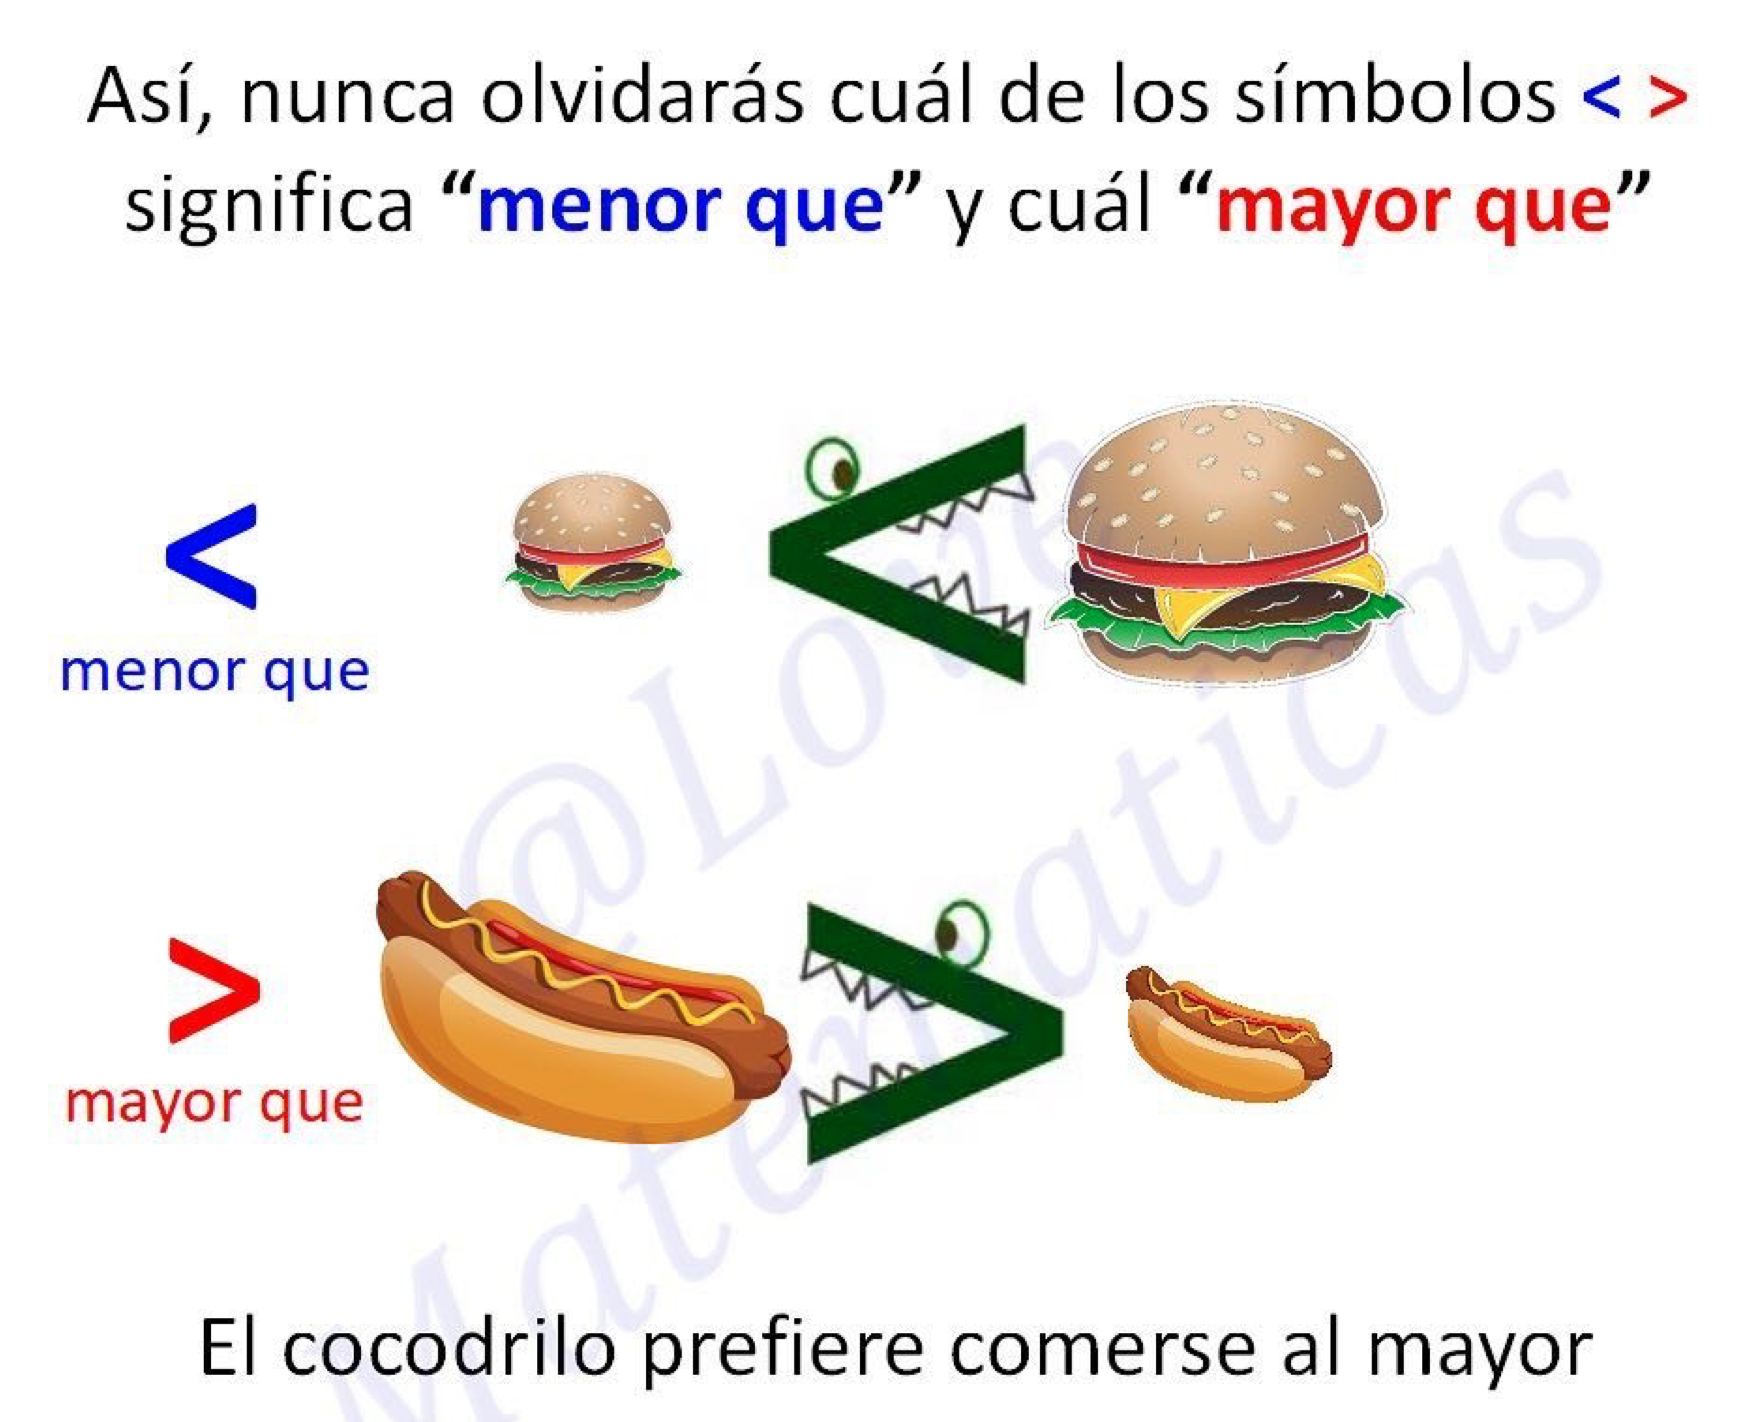
\includegraphics[width=0.45\textwidth]{img-ecc/ecc10.png}
	\end{figure}
\end{multicols}




\vspace{1cm}
\section{Inecuaciones con una incógnita}

\begin{tikzpicture}
	\fill [left color=red!50, right color=teal!50] (0,0) rectangle (3.5,.1);
	\fill [left color=teal!50, right color=blue!50] (3.5,0) rectangle (7.5,.1);
	\end{tikzpicture}
\vspace{0.5cm}

\subsection{Inecuaciones lineales con una incógnita}
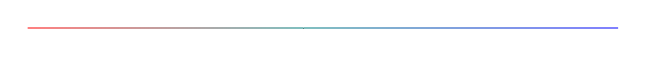
\begin{tikzpicture}
	\fill [left color=red!50, right color=teal!50] (0,0) rectangle (3.5,.01);
	\fill [left color=teal!50, right color=blue!50] (3.5,0) rectangle (7.5,.01);
	\end{tikzpicture}
\vspace{0.5cm}

\begin{definition}

Tienen la forma: $\qquad ax+b \ < 0 \ (\leqslant, >, \geqslant)\  , \ \text{ con } a,b\in \mathbb R,\ a\neq 0$
	
\end{definition}

\begin{theorem}

Procedimiento de resolución:

\begin{itemize}
\vspace{-2mm} \item Quitar paréntesis.
\vspace{-2mm} \item Quitar denominadores.
\vspace{-2mm} \item Trasponer términos.
\vspace{-2mm} \item Reducir a términos semejantes.
\vspace{-2mm} \item Despejar (cuidado: si hay que multiplicar --dividir-- por un número negativo, la desigualdad se invierte --cambia de sentido--)	
\end{itemize}
	
\end{theorem}

\begin{miejemplo}

	Resuelve $\qquad \dfrac 2 3 \left[ x-\left( 1-\dfrac{x-2}{3} \right) \right]+1\ <\ x$
	
\vspace{5mm} $\dfrac 2 3 \left[ x- 1+\dfrac{x-2}{3}  \right]+1\ <\ x
\ \to \ 
\dfrac 2 3 \left[ \dfrac{3x-3+x-2}{3}  \right]+1\ <\ x \ \to \ 
\dfrac 2 3 \left[ \dfrac{4x-5}{3}  \right]+1 \ \to $

\vspace{2mm} $\to \textcolor{red}{9\, }\cdot \dfrac{2(4x-5)}{9} + \textcolor{red}{9\, }\cdot 1 < \textcolor{red}{9\, }\cdot x \, ; \ \ \text{MCD: \textcolor{red}{9\, }} \ \to \ 2(4x-5)+9<9x\ \to 8x-10+9<9x \to $

\vspace{2mm}$\to \ 8x-9x<10-9 \ \to \ -x<1\, ;\quad  \text{ multiplicando por } (-1) \ \Rightarrow \ \boldsymbol{x>-1}$

\vspace{2mm} Solución: $\ \{ \forall x \in \mathbb R \, / \, \ x>-1 \}\ \longleftrightarrow \ \ \boldsymbol{]-1,+\infty[}$
\end{miejemplo}

\begin{miejercicio}

Resuelve: $\qquad 6\left( \dfrac{x+1}{8}-\dfrac{2x-3}{16} \right) \ \geqslant \ 3\left( \dfrac{3}{4}x-\dfrac 1 4 \right) - \dfrac 3 8 (3x-2)$

\rule{250pt}{0.1pt}	

\vspace{5mm} $\dfrac{6(x+1)}{8}-\dfrac{6(2x-3)}{16} \geqslant \dfrac{3(3x-1)}{4}-\dfrac{3(3x-2)}{8};\qquad MCM:16$

\vspace{2mm} $16\cdot \dfrac{6(x+1)}{8}-16\cdot \dfrac{6(2x-3)}{16} \geqslant 16\cdot \dfrac{3(3x-1)}{4}-16\cdot \dfrac{3(3x-2)}{8}$

\vspace{2mm} $12(x+1)-6(2x-3) \geqslant 12(3x-1)-6(3x-2) \ \to \ \cancel{12x}]+12-\cancel{12x}+18 \leqslant 36x-\cancel{12}-18x+\cancel{12}$

\vspace{2mm} $-36x+18x \geqslant -12-18 \ \to \ -18x \geqslant 30\, ; \ $ Multiplicando por $\, (-1)$:

\vspace{2mm} $18 \leqslant -30 \ \to \ x\leqslant 5/3\ \ $ Solución: $\ \{ \forall x \in \mathbb R \, / \, \ x \leqslant 5/3 \}\ \longleftrightarrow \ \ \boldsymbol{]-\infty,5/3]}$

\end{miejercicio}


\vspace{0.5cm}
\subsection{Inecuaciones no lineales con una incógnita}
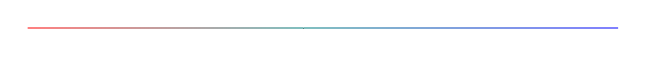
\begin{tikzpicture}
	\fill [left color=red!50, right color=teal!50] (0,0) rectangle (3.5,.01);
	\fill [left color=teal!50, right color=blue!50] (3.5,0) rectangle (7.5,.01);
	\end{tikzpicture}
\vspace{0.5cm}

No es sencillo estudiar cuando una determinada expresión algebraica es mayor (o menor) a otra, pero resulta más sencillo estudiar cuado una determinada expresión es mayor (menor) que cero, cuando es positiva (o negativa), cuando cambia de signo (en algún momento ha de valer cero). Por ello esta será la estrategia principal que usaremos: \emph{llevar todo a un solo miembro de la inecuación y en el otro habrá un cero}, determinaremos cuando es cero el numerador y denominador de nuestra expresión (si los hay) y estudiaremos el signo que toma la expresión a estudio en cada una de las zonas que aparecerán. 

Para inecuaciones irracionales con radicales pares hay que exigir, además, que todos los radicandos sean no negativos ($\geqslant 0$). Las inecuaciones sobre valores absolutos serán más delicadas, veremos todo esto en ejemplos y ejercicios resueltos a continuación.

\vspace{5mm}
\begin{large}
$\triangleright \quad $ \textbf{Inecuaciones de segundo grado}	
\end{large}
\vspace{5mm}

\begin{miejemplo}

Resuelve la inecuación: $\qquad 6x^2 \geqslant 5x+6$

\vspace{5mm} $6x^2-5x-6\geqslant 0 \ \longrightarrow	 \ 6x^2-5x-6=0 \ \leftrightarrow \ x=3/2 \ \wedge \ x=-2/3$

\vspace{2mm} $6x^2-5x-6=6(x-3/2)(x+2/3)=2(x-3/2)3(x+2/3)=(2x-3)(3x+2)$

\vspace{2mm} Nuestra inecuación es: $\quad (2x-3)(3x+2) \geqslant 0	\, ; \ $ Sabemos que es cero en $-2/3$ y en $3/2$, por lo que dividiremos el eje real en 3 zonas (y dos puntos) en que estudiaremos el signo que toma nuestra expresión \textcolor{gris}{(números menores que -2/3, en -2/3, desde -2/3 hasta 3/2, en 3/2, números mayores que 3/2)}.

\begin{table}[H]
\centering
\begin{tabular}{c|c|c|c|c|c|}
 & $]-\infty,-2/3[$  & $x=-2/3$ & $]-2/3,3/2[$ & $x=3/2$ & $]3/2,+\infty$[ \\ \hline
2x-3 & $-$ & $-$ & $-$ & 0 & $+$ \\ \hline
3x+2 & $-$ & 0 & $+$  & $+$  & $+$  \\ \hline
(2x-3)(3x+2) & $+$  & 0 & $-$	 & 0 & $+$  \\ \hline
?`$6x^2-5x-6 \geqslant 0$? & Sí & Sí  & No & Sí & Sí \\ \hline
\end{tabular}
\end{table}

Los signos los obtenemos al sustituir un número cualquiera de la zona en cuestión en la expresión indicada; así, p.e. en la zona $]-\infty,-2/3[$ tomamos el valor $x=-1$, el factor $2x-3=2(-1)-3=-5<0$, es negativo, $\boldsymbol{-}$. El factor $3x+2=3(-1)+2=-1<0$, también lo es, por lo que el producto $(2x-3)(3x+2)$ será positivo, $\boldsymbol{+}$ en esta zona.

Solución: $\boldsymbol{]-\infty,-2/3]\cup[3/2,+\infty[}$

\end{miejemplo}

\begin{multicols}{2}

Gráficamente: 

$\ y=x^2-5x-6=0\ $ es una parábola que corta al eje $\mathcal OX$ en $A(3/2,0)$ y $B(-2/3,0)$.

Una vez representada se observa que la parábola es positiva ($y\geqslant 0$) en $\ ]-\infty,-2/3]\cup[3/2,+\infty[$
\begin{figure}[H]
		\centering
		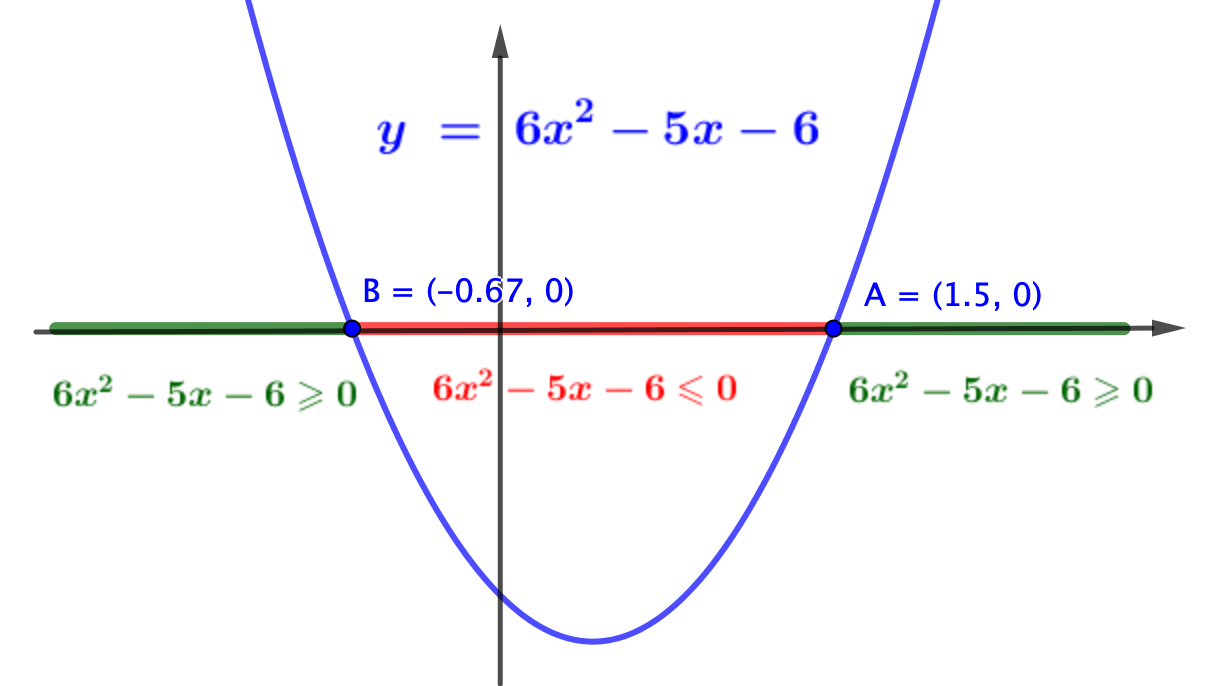
\includegraphics[width=0.5\textwidth]{img-ecc/ecc11.png}
	\end{figure}	
\end{multicols}

\begin{miejercicio}

Resuelve: $\qquad a)\ \ x^2+4x+4\leqslant 0;\qquad \qquad b)\ \ x^2+1\leqslant x$

\rule{250pt}{0.1pt}

\vspace{5mm} $\triangleright \quad a)\ \ x^2+4x+4=0 \ \to \ x=-2$

\vspace{2mm} Tenemos un único punto, dará lugar a tres zonas: menores que -2, el número -2 y mayores que -2. En ellas estudiaremos el signo que toma $x^2+4x+4$. 

\vspace{2mm} Con una tabla similar a la anterior obtendríamos que $x^2+4x+4$ es positivo (mayor que cero) tanto para números mayores que -2 como para números menores que -2 y que vale 0 en x=-2, por lo que la solución buscada, cuando $x^2+4x+4\leqslant0$, cuando es negativa o cero es, únicamente, para x=2. Solución, $\boldsymbol{x=2}$

\vspace{2mm} Pero es más sencillo razonar: $x^2+4x+4=0 \leftrightarrow x=-1 \ \to \ x^2+4x+4=(x+2)^2$ que \textbf{siempre} es positivo o cero, por lo que será $x^2+4x+4=(x+2)^2\leqslant 0$ solamente en $\boldsymbol{x=-2}$

\vspace{2mm} Para la inecuación $x^2+4x+4<0$, la solución sería $\nexists x$, que no la hay. Si la inecuación fuese $x^2+4x+4\geqslant 0$, la solución sería todos los números reales, $\mathbb R$. Y si la inecuación hubiese sido $x^4+4x+4>0$, la solución sería $]-\infty,-2[	\cup ]-2,+\infty[$

\vspace{5mm} $\triangleright \quad b) \ \ x^2+1\leqslant x \ \to \ x^2-x+1 \leqslant 0 \quad $ Veamos cuando es cero:

\vspace{2mm} $x^2-x+1=0 \ \to \ x=\dfrac{1\pm \sqrt{(-1)^2-4\cdot 1 \cdot 1}}{2} \ \ \nexists\ $  

\vspace{2mm} $x^2-x+1$ nunca es cero, nunca pasa por el cero, luego o siempre será positivo o siempre negativo. Tomemos un número cualquiera, p.e. $x=0 \to \ 0^2+4\cdot 0 + 4=4 > 0\, . \ $ Esta expresión es \emph{siempre} positiva, por lo que $x^2-x+1\leqslant 0$ nunca. Solución: $\ \emptyset   \ $ (conjunto vacío).

\vspace{2mm} También podríamos haber hecho una tabla con una sola zona, $\mathbb R$, el signo en esta. zona lo obtenemos al sustituir cualquier número de esta zona en nuestra inecuación y comprobar que  p.e. $x=0 \to \ 0^2+4\cdot 0 + 4=4 > 0\, . \ $, por lo que la inecuación no tendría solución.

\end{miejercicio}

\vspace{5mm}
\begin{large}
$\triangleright \quad $ \textbf{Inecuaciones de grado superior a 2}	
\end{large}
\vspace{5mm}

Se tratan del mismo modo que las de segundo grado

\begin{miejercicio}

Resuelve $\qquad x^4-20x \ \geq \ x^3+16x^2$

\rule{250pt}{0.1pt}	

\vspace{5mm} Llevando todo a la izquierda: $\ \ x^4-x^3-16x^2-20x \ \leqslant \ 0$

\vspace{2mm} Sacando factor común y factorizando, $\ x(x-5)(x+2)^2 >0\ $ \textcolor{gris}{El factor $(x+2)^2$ siempre es positivo por lo que solo puede cambiar el signo a la izquierda y derecha del 0 y del 5, el -2 no alterará los signos, salvo que dará 0 en x=-2. De todos modos, como se trata de un ejercicio para ilustrar el método no lo tendremos en cuenta.}

\vspace{2mm} Buscamos los ceros que darán lugar a las zonas en que estudiaremos los signos de los factores: $\ x(x-5)(x+2)^2=0 \ \leftrightarrow \ x=0\ \wedge \ x=5 \ \wedge \ x=-2$

\begin{table}[H]
\centering
\begin{tabular}{c|c|c|c|c|c|c|c|}
 & $]-\infty,-2[$ & $-2$ & $]-2,0[$ & $0$ & $]0,5[$ & $5$ & $]5,+\infty[$ \\ \hline
$x$            & $-$ & $-$ & $-$ & 0 & $+$ & $+$ & $+$ \\ \hline
$x-5$          & $-$ & $-$ & $-$ & $-$ & $-$ & 0 & $+$ \\ \hline
$(x+2)^2$.     & $+$ & 0 & $+$ & $+$ & $+$ & $+$ & $+$ \\ \hline
$x(x-5)(x+2)^2$ & $+$ & 0 & $+$ & 0 & $-$ & 0 & $+$ \\ \hline
?`$x(x-5)(x+2)^2\geqslant 0$? & No & Sí & No & Sí & Sí & Sí & No \\ \hline
\end{tabular}
\end{table}
Solución: $\quad \boldsymbol{ \{-2\} \cup [0,5]}$

\vspace{2mm} Si la inecuación hubiese sido, por ejemplo, $x^2+20x<x^3+16x*2$, cuando se obtiene un resultado negativo (no cero), la solución sería $\ ]0,5[$
\end{miejercicio}


\vspace{5mm}
\begin{large}
$\triangleright \quad $ \textbf{Inecuaciones sobre fracciones algebraicas}	
\end{large}
\vspace{5mm}

En este tipo de inecuaciones aparecerá, como novedad, que si el cero procede de un factor del denominador, al no estar definida la división por cero en matemáticas, proporcionará un punto donde la fracción no existirá, por lo que jamás formará parte de la solución.


\begin{miejemplo}

Resuelve: $\qquad \dfrac{x-1}{3x+6}>0$	

\vspace{5mm} Ceros numerador: $\ x-1=0 \ \to \ x=1\, . \ $ Ceros denominador $\ 3x+6=0 \ \to \ x=-2 \, . \ $ Los números 1 y -2 dividen en eje real en tres zonas (menores que -2, entre -2 y 1, mayores que 1):

\begin{table}[H]
\centering
\begin{tabular}{c|c|c|c|c|c|}
 & $]-\infty,-2[$ & $x=-2$ & $]-2,1[$ & $x=1$ & $]1,+\infty[$ \\ \hline
$x-3$ & $-$ & $-$ & $-$ & $0$ & $+$ \\ \hline
$3x+6$ & $-$ & $0$ &$+$  & $+$ & $+$ \\ \hline
$\dfrac{x-1}{3x+6}$ &$+$  & $\nexists$ & $-$ & $0$ & $+$ \\ \hline
?`$\ \dfrac{x-1}{3x+6}>0\ $? & Sí & No & No & No & Sí \\ \hline
\end{tabular}
\end{table}

Solución: $\quad ]-\infty,-2[ \ \cup \ ]1,+\infty[$

\end{miejemplo}

\begin{miejercicio}

Resuelve: $\qquad \dfrac{x^3+3x^2+x-4}{x^3+2x^2+x} \leqslant 1$

\rule{250pt}{0.1pt}

\vspace{4mm} Antes de buscar los ceros de numerador y denominador tenemos que tener todo a la izquierda y cero a la derecha (para poder estudiar signos)

\vspace{2mm} $\dfrac{x^3+3x^2+x-4}{x^3+2x^2+x} \leqslant 1 \quad \to \quad \dfrac{x^3+3x^2+x-4}{x^3+2x^2+x} -1\leqslant 0 \ \to $

\vspace{2mm} $\to \ \dfrac{x^3+3x^2+x-4-(x^3+2x^2+x)}{x^3+2x^2+x}\leqslant 0 \quad \to \quad \dfrac{x^2-4}{x^3+2x^2+x} \leqslant 0 $

\vspace{2mm} Ceros numerador: $\ x^2-4=0 \to x=2,\ x=-2;\ $ ceros denominador $\ x(x^2+x+1)=0 \to x=0\quad $ \textcolor{gris}{$(x^2+x+1\neq 0)\quad $}  Hemos de cortar la recta real en -2, 0 y 2.

\vspace{2mm} Nuestra inecuación (factorizada, que es mejor para estudiar signos) queda como: $\quad \dfrac{(x-2)(x+2)}{x(x^2+x+1)}\leqslant 0$

\begin{table}[H]
\centering
\begin{tabular}{c|c|c|c|c|c|c|c|}
 & $]-\infty,-2[$  & $-2$ & $]-2,0[$ & $0$ & $]0,2[$ & $2$ & $]2,+\infty[$ \\ \hline
$(x-2)$ & $-$ & $-$ & $-$ & $-$ & $-$ & $0$ & $+$ \\ \hline
$(x+2)$ & $-$ & $0$ & $+$ & $+$ & $+$ & $+$ & $+$ \\ \hline
$x$ & $-$ & $-$ & $-$ & $0$ & $+$ & $+$ & $+$ \\ \hline
$x^2+x+1$ & $+$ & $+$ & $+$ & $+$ & $+$ & $+$ & $+$ \\ \hline
$\dfrac{(x-2)(x+2)}{x(x^2+x+1)}$ & $-$ & $0$ & $+$ & $\nexists$ & $-$ & $0$ & $+$ \\ \hline
?`$\ - \text{ o } 0\ $? & Sí & Sí & No & No & Sí & Sí & No \\ \hline
\end{tabular}
\end{table}

\vspace{2mm} Solución: $\quad ]-\infty,-2]\ \cup \ ]0,2]$
	
\end{miejercicio}

\vspace{5mm}
\begin{large}
$\triangleright \quad $ \textbf{Inecuaciones con raíces cuadradas}	
\end{large}
\vspace{5mm}

Ahora, además de verificarse la inecuación que nos planteen, tenemos que exigir que los radicandos sean no negativos (positivos o cero, $\geqslant 0$).

\begin{miejemplo}

Resuelve: $\qquad \sqrt{3x-2} < 5$

\vspace{5mm} $\begin{cases}
 \	\exists \sqrt{3x-2} \ \to \ 3x-2\geqslant 0 \ \to \ x\geqslant 2/3
 \ \Rightarrow \ [2/3,+\infty[ \\
 \ \sqrt{3x-2} < 5 \ \to \ 3x-2<5^2=25 \ \to \ 3x<27 \ \to x<9 \ \Rightarrow \ ]-\infty, 9[ 	\end{cases}$

 
\begin{multicols}{2} 
Las dos condiciones se cumplirán a la vez en la intersección de los intervalos obtenidos:  

\begin{figure}[H]
		\centering
		
\includegraphics[width=0.5\textwidth]{img-ecc/ecc12.png}
	\end{figure}	
\end{multicols}

\vspace{-4mm}$[2/3,+\infty[ \ \cap \ ]-\infty,9] \ \Rightarrow \ $ Solución: $\quad [2/3,9[$ 

\vspace{2mm}\begin{small} \textcolor{gris}{Hemos dibujado un intervalo de rojo y otro de azul, la intersección aparece en morado.}	 \end{small}
\end{miejemplo}

\begin{miejercicio}

Resuelve: $\qquad \sqrt{3x^2-17x+10} \ \leqslant\ 4$

\rule{250pt}{0.1pt}

\vspace{4mm} $\triangleright \quad$ Por un lado, $\quad \exists 	\sqrt{3x^2-17x+10}  \ \leftrightarrow \ 3x^2-17x+10 \geqslant 0 \quad (*)$

\vspace{2mm} $\triangleright \quad$ Por otro lado, $\quad  	\sqrt{3x^2-17x+10}\leqslant 4  \ \leftrightarrow \ 3x^2-17x+10  \leqslant 16 \quad (**)$

\vspace{4mm} --- Condición $(*) \quad 3x^2-17x+10 \geqslant 0 $

\vspace{2mm} $3x^2-17x+10=0 \ \to \ x=5 \ \wedge \ x=2/3 \ \to 3x^2-17x+10=3(x-5)(x-2/3)$

\vspace{2mm} Nuestra condición $(*)$ exige que $\quad (x-5)(3x-2)\geqslant 0$

\vspace{2mm} Estudiando los signos en las zonas: menores que 2/3, en 2/3, desde 2/3 hasta 5, en 5 y mayores que 5 en un atabla como venimos haciendo hasta ahora, encontraremos que 

\vspace{2mm} $(x-5)(3x-2)\geqslant 0 \quad \Rightarrow \quad ]-\infty, 2/3]\cup[5,+\infty[$

\vspace{4mm} --- Condición $(**)\quad 3x^2-17x+10  \leqslant 16$

\vspace{2mm} $3x^2-17x+10  \leqslant 16 \ \to 3x^2-17x+10-16 =3x^2-17x-6 \leqslant 0$

\vspace{2mm} $3x^2-17x-6=0 \ \to \ x=6 \ \wedge \ x=-1/3 \ \to 3x^2-17x-6=3(x-6)(x+1/3)$

\vspace{2mm} Nuestra condición $(**)$ exige que $\quad (x-6)(3x+1)\leqslant 0$

\vspace{2mm} Procediendo como en el caso anterior y cortando al eje real en $6$ y $-1/3$ para estudiar signos, se obtiene que
$\quad (x-6)(3x+1)\leqslant 0 \ \Rightarrow \ [-1/3,6]$

\vspace{4mm} Las condiciones $(*)$ y $(**)$ se cumplirán. a la vez en la intersección de los intervalos obtenidos:

\begin{multicols}{2}
$ \left( \ ]-\infty, 2/3]\cup[5,+\infty[ \ \right) \ \cap \  [-1/3,6] $

\begin{center}$[-1/3,2/3] \ \cup \ [5,6]$\end{center}
	\begin{figure}[H]
		\centering
		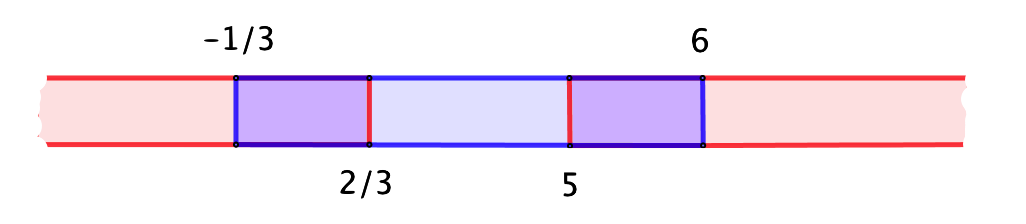
\includegraphics[width=0.5\textwidth]{img-ecc/ecc13.png}
	\end{figure}
\end{multicols}
\begin{small} \textcolor{gris}{Hemos dibujado unos intervalos de rojo y otro de azul, las intersecciones aparecen en morado.}	 \end{small}
\end{miejercicio}


\vspace{3mm}
\begin{large}
$\triangleright \quad $ \textbf{Inecuaciones con valor absoluto}	
\end{large}
\vspace{2mm}

\begin{adjustwidth}{50pt}{50pt}
\begin{destacado}
\begin{table}[H]
\centering
\begin{tabular}{lcc}
$|x|<a$ & $-a<x<a$ & $]-a,a[$ \\
$|x|\leqslant a$ & $-a\leqslant x \leqslant a$ & $[-a,a]$ \\
$|x|>a \quad $ & $\quad  x<-a \ \vee \ x>a \quad $ & $\quad ]-\infty,-a[ \ \cup \ ]a,+\infty[$ \\
$|x|\geqslant a \quad $ & $ \quad x \leqslant -a \ \vee \ x \geqslant a \quad $ & $\ \quad ]-\infty,-a] \ \cup \ [a,+\infty[$
\end{tabular}
\end{table}
\vspace{-10mm}
\end{destacado}
\end{adjustwidth}

\begin{miejemplo}
	
	Resuelve: $\qquad |2x-6| \ < \ 4$

\vspace{4mm} $-4<2x-6<4 \ \to \ \begin{cases}
 \ 2x-6<4 \ \to 2x<10 \ \to \ x<5 \\ \ -4<2x-6 \to \ 2<2x \ \to 1<x	
 \end{cases} \ \Rightarrow 1<x<5$
 
 \vspace{2mm} Solución: $\quad ]1,5[$



\end{miejemplo}

\begin{miejercicio}
	. Resuelve $\qquad |3x+1| \ \geqslant \ 5$
	
\rule{250pt}{0.1pt}

\vspace{4mm} $\begin{cases} \ 3x+1\geqslant 5 &\to x\geqslant 4/3 \\ \ 3x+1\leqslant -5 &\to x\leqslant -2 \end{cases} \ \to x\geqslant 4/3 \ \vee \ x\leqslant -2 \ \Rightarrow \ \text{solución: } \ ]-\infty,-2] \ \cup \ ]4/3,+\infty[$
\end{miejercicio}


%%%%%%%%%%%%%%%%%%%%%%%%%%%%%%%%%
\begin{miejercicio}
	. Resuelve: $\qquad |x^2+3|=5;\qquad |x^2+3|<5; \qquad |x^2+3|\ge 5$
	
\rule{250pt}{0.1pt}
		
		
\vspace{4mm} * $-5=x^2+3=5 \to 
			\left\{ 
			\begin{matrix} 
				x^2+3=-5\quad \to \quad x^2=-8 \to \quad \nexists x\\ 
				x^2+3=5\quad \to \quad x^2=2 \quad \to |x|=\sqrt 2 
				\end{matrix} 
				\right.$  
				
\vspace{2mm} Solución: $x=\sqrt 2\; \vee \; x=-\sqrt2$
				
\vspace{4mm}  ** $-5<x^2+3<5 \to -8<x^2<2$. La primera desigualdad no aporta nada, ya que $-8<x^2$ lo cumplen todos los números reales. Para la segunda, $x^2<2$, llevaremos todos los términos a la izquierda: $x^2-2<0$ y buscaremos los ceros de 
				$x^2-2$. 

\begin{multicols}{2}				
\vspace{2mm} $x^2-2=0 \to x=\sqrt 2 \; \vee \; x=-\sqrt 2\ $ 

\vspace{2mm} Dividiendo el eje real en 3 zonas, como muestra la siguiente figura, obtenemos la solución: $]-\sqrt 2;\, \sqrt 2[$
				
			\begin{figure}[H]
			\centering
				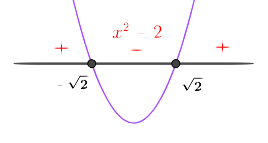
\includegraphics[width=0.4\textwidth]{img-ecc/ecc14.png}
			\end{figure}
\end{multicols}				

\vspace{-4mm}  *** $|x^2+3|\ge 5 \quad \to \quad x^2+3\le -5: \; x^2\le -8; \; \nexists x \qquad  \vee \qquad  x^2+3\ge 5: \; x^2\ge 2; \; x^2-2\ge 0$ De donde, procediendo como en el caso anterior para estudiar el signo de $x^2-2$ viendo previamente cuando $x^2-2=0$ y representando en $\mathbb R$ para estudiar los signos que toma $x^2-2$, usando la misma figura anterior, obtenemos como solución: $]-\infty, -\sqrt 2]\; \cup \; [\sqrt 2, \infty[$
\end{miejercicio}


\begin{miejercicio}
	. Resuelve $\qquad \left| \dfrac {3x+12}{x+2} \right| \ge 1$

\rule{250pt}{0.1pt}
		
\vspace{5mm} Establezcamos primero que en ningún momento podemos admitir la solución $x=-2$ puesto que anula un denominador de la inecuación de partida.
			
\vspace{2mm} $\left| \dfrac {3x+12}{x+2} \right| \ge 1 \to \dfrac {3x+12}{x+2} \le -1 \; (i)\quad \vee \quad \dfrac {3x+12}{x+2} \ge 1 \; (ii)$
			
\vspace{2mm} Resolveremos las dos inecuaciones $(i)$ e $(ii)$ por separado y tomaremos como solución la unión de las mismas, excluyendo al $-2$ si está en ellas.
 
 \vspace{2mm} Inecuación $(i): \quad \dfrac {3x+12}{x+2} \le -1 \to \dfrac {3x+12}{x+2} +1\le 0 \to \dfrac {4x+14}{x+2} \le 0$		
 			
 \vspace{2mm} Los ceros de esta expresión son $x=-7/2$ y $x=-2$ que dictarán los intervalos en que estudiar el signo del cociente. Lo vemos en la siguiente tabla:
 					
 			\begin{table}[H]
 			\centering
			\begin{tabular}{|c|c|c|c|c|c|}
			\hline
 			Intervalos&$]-\infty,-7/2[$  &$-7/2$  &$]-7/2,-2[$  & $-2$ &$]-2,\infty[$ \\ \hline
 			$4x+14$& $-$ & 0 & + &+  & +\\ \hline
 			$(x+2)$& $-$ & $-$  & $-$  &0  & +\\ \hline
 			$\dfrac {4x+14}{x+2}$& + & 0 & $-$ & $\nexists$ & +\\ \hline
			\end{tabular}
			\end{table}
			
Solución $(i):\qquad [-7/2,2[$
			
\vspace{2mm} Inecuación $(ii): \quad \dfrac {3x+12}{x+2} \ge 1 \to \dfrac {3x+12}{x+2} -1\ge 0 \to \dfrac {2x+10}{x+2} \ge 0$	
			
\vspace{2mm} Los ceros de esta expresión son $x=-5$ y $x=-2$ que dictarán los intervalos en que estudiar el signo del cociente. Lo vemos en la siguiente tabla:
 				
 			\begin{table}[H]
 			\centering
			\begin{tabular}{|c|c|c|c|c|c|}
			\hline
 			Intervalos&$]-\infty,-5[$  &$-5$  &$]-5,-2[$  & $-2$ &$]-2,\infty[$ \\ \hline
 			$2x+10$& $-$ & 0 & + &+  & +\\ \hline
 			$(x+2)$& $-$ & $-$  & $-$  &0  & +\\ \hline
 			$\dfrac {2x+10}{x+2}$& + & 0 & $-$ & $\nexists$ & +\\ \hline
			\end{tabular}
			\end{table}
 			
 Solución $(ii):\qquad ]-\infty,-5]\;  \cup \;  ]-2,\infty[$
 			
 \vspace{2mm} Finalmente, la solución del problema la formarán la unión de los intervalos solución $(i)$ y $(ii)$, excluyendo, si es necesario al $\{ -2 \}$:
 			
\vspace{2mm}  Solución:  $]-\infty, -5] \; \cup\;  [-7/2, -2[ \; \cup\;  ]-2, \infty[$

\end{miejercicio}

\vspace{0.5cm}
\section{Sistemas de inecuaciones con una incógnita}

\begin{tikzpicture}
	\fill [left color=red!50, right color=teal!50] (0,0) rectangle (3.5,.1);
	\fill [left color=teal!50, right color=blue!50] (3.5,0) rectangle (7.5,.1);
	\end{tikzpicture}
\vspace{0.5cm}

Cada inecuación dará lugar a unos intervalos solución. 

La solución de todo el sistema será la intersección de los intervalos soluciones de cada una de las inecuaciones que conforman el sistema.

\vspace{4mm}
\begin{miejemplo}

Resuelve $\qquad \begin{cases} \ 2x+3 \geqslant -x-3 \\ \ 2(x-1) \leqslant x+4 \end{cases} $

\vspace{5mm} $\left. \begin{array}{lll} 3x\geqslant 6 & \to \ x\geqslant -2 &\to \ [-2,+\infty[ \\ 2x-2\leqslant x+4 & \to \ x\leqslant 6 &\to \ ]-\infty,6] \end{array} \right\} \ \Rightarrow \ [-2,+\infty[ \ \cap \ ]-\infty,6] \ = \ [-2,6]$

\end{miejemplo}

\begin{miejercicio}

Resuelve $\qquad \begin{cases} \ x^2-4x-21 >0\\ \ 4-2x \leqslant 6 \end{cases}$	

\vspace{2mm}
\rule{250pt}{0.5pt}

\vspace{5mm} $\left. \begin{array}{lll} 
	x^2-4x-21 > 0 &\to \ (x-7)(x-3)<0 &\to \ ]-3,7[\ (*) \\
	4-2x\leqslant 6 &\to \ -2x\leqslant 2 \to x\geqslant -1 &\to \ [-1,+\infty[
 \end{array}\right\} \  \Rightarrow $
 
 \vspace{2mm} $\Rightarrow \  ]-3,7[ \ \cap [-5,+\infty[ \ = \ [-1,7[$

\vspace{2mm} \begin{small} \textcolor{gris}{La solución ($*$) la hemos obtenido mediante una tabla o razonando: se trata de una parábola hacia arriba que corta al eje $\mathcal OX$ en -3 y 7, será negativa entre los cortes.} \end{small}

\vspace{2mm} 	
\end{miejercicio}

\begin{miejercicio}

Resuelve $\qquad \begin{cases} \ x^2-2x-8\leqslant 0 \\ \ \dfrac{x-1}{x+1} > 0 \end{cases}$	

\vspace{2mm}

\rule{250pt}{0.5pt}

\vspace{5mm} La primera inecuación es, factorizada, $\ (x-4)(x+2)\leqslant 0\, , \  $ que es positiva o cero en $[-2,4].\ $ \textcolor{gris}{Basta con construir una tabla donde estudiar los signos de los factores de la descomposición o razonar donde la parábola es no positiva (negativa o cero).}

\vspace{4mm} La segunda inecuación es racional, con ceros de numerador y denominador en 1 y -1, respectivamente. La solución a esta inecuación es $]-\infty,-1[\ \cup\ ]1,+\infty[.\ $ \textcolor{gris}{Constrúyase la tabla adecuada para el estudio del signo de la fracción.}

\vspace{4mm} La solución estará en la intersecciones de las soluciones de las inecuaciones:

\vspace{2mm} $[-2,4] \cap \ \left( \ ]-\infty,-1[\ \cup\ ]1,+\infty[ \ \right) \ = \ [-2,-1[ \ \cup \ ]1,4]$

\vspace{2mm} 	
\end{miejercicio}

\vspace{1cm}
\section{Inecuaciones lineales con dos incógnitas}

\begin{tikzpicture}
	\fill [left color=red!50, right color=teal!50] (0,0) rectangle (3.5,.1);
	\fill [left color=teal!50, right color=blue!50] (3.5,0) rectangle (7.5,.1);
	\end{tikzpicture}
\vspace{0.5cm}



\begin{theorem}
.	Una ecuación lineal con dos incógnitas $ \ \boldsymbol{ax+by=c} \ $ es una \textbf{recta} en el plano.
\end{theorem}

\begin{figure}[H]
	\centering
	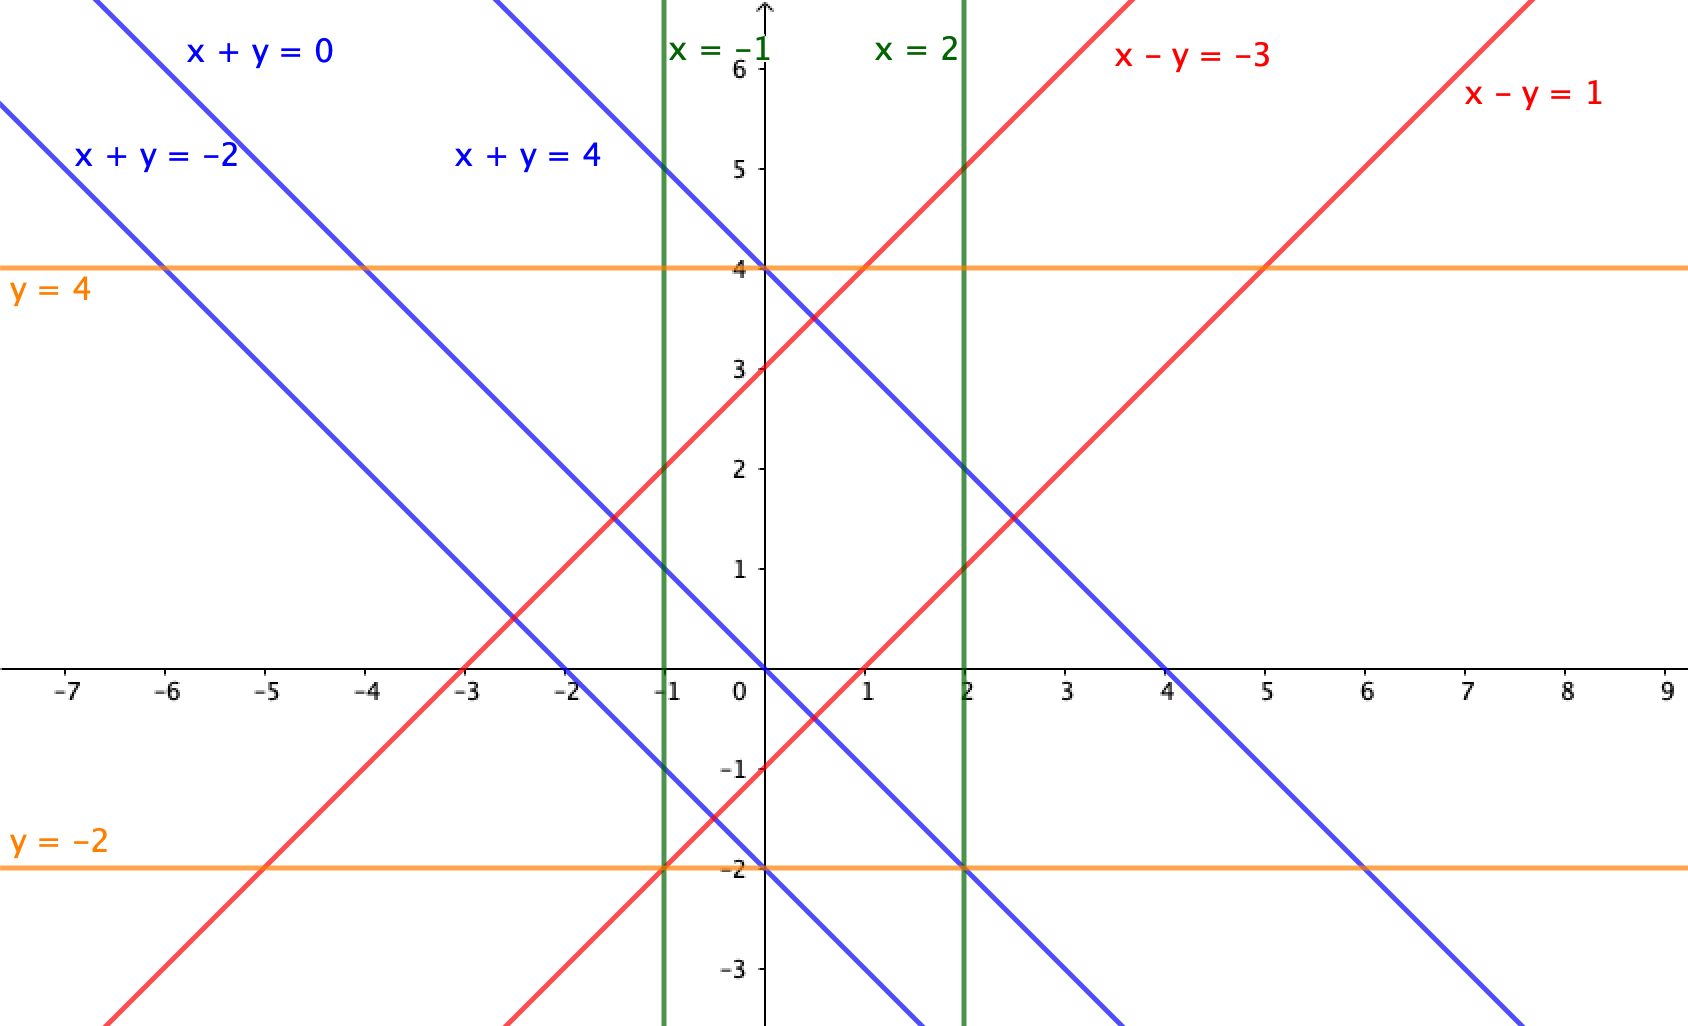
\includegraphics[width=.9\textwidth]{imagenes/img05.png}
\end{figure}

\vspace{5mm}
\begin{theorem}
.	Una \textbf{inecación} lineal con dos incógnitas $ \ \boldsymbol{ax+by \le c} \ $ es una desigualdad: $\ <,\ \le, \ >,\ \ge\ $ y se corresponde con un \textbf{semiplano} a uno de los lados de la recta (que es donde se verifica la igualdad, $=$).

\vspace{5mm}
\begin{destacado}
	Para averiguar cual de los dos semiplanos en que una recta divide al plano es la que representa a la inecuación dada, elegimos un punto en uno de los dos semiplanos (que no pertenezca a la recta)\footnote{Si el punto elegido es de la recta, lo que se verifica es la ecuación: ``la recta son los puntos del plano que verifican su ecuación''} y sustituimos sus coordenadas en la inecuación; si ésta se cumple, estamos en la zona adecuada; si no es así, la inecuación representa al otro semiplano.
\end{destacado}
\end{theorem}

\begin{figure}[H]
	\centering
	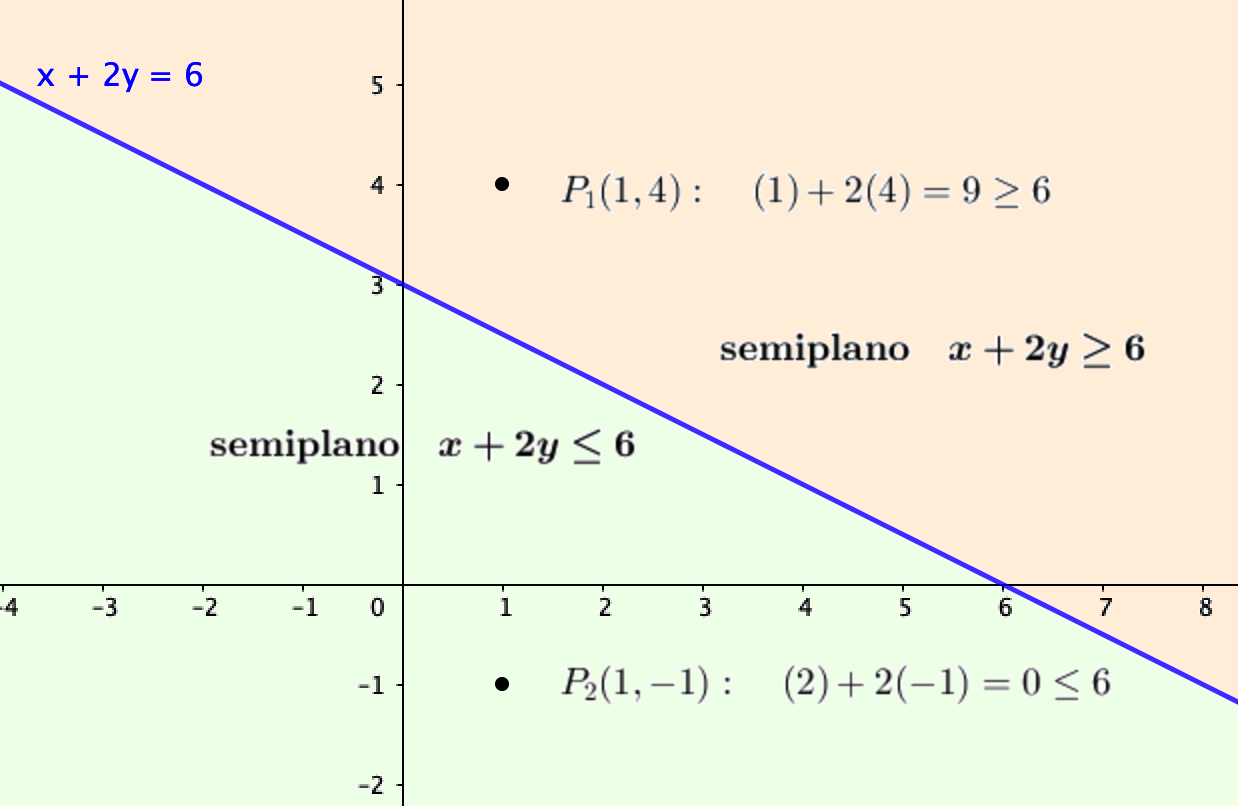
\includegraphics[width=.75\textwidth]{imagenes/img06.png}
\end{figure}

\vspace{5mm}
El semiplano solución puede ser \textbf{abierto} si no contiene a la recta, responde a una inecuación estricta ($<,\ >$); o \textbf{cerrado} si sí contiene a la recta, responde a inecuaciones no estrictas ($\le,\ \ge$). En el caso de semiplanos abiertos, dibujaremos la recta que los limita de forma discontinua.

\vspace{5mm}
\begin{destacado}
$\ $

Para resolver una inecuación,

\begin{adjustwidth}{20pt}{10pt}
\vspace{4mm} $\triangleright \ $ Primero representaremos la recta (sustituimos la desigualdad por un signo igual) mediante una tabla de valores, bastará con buscar dos de sus puntos.

\vspace{4mm} $\triangleright \ $ Elegimos un punto cualquiera que no esté en la recta y verificamos si ese punto cumple o no la inecuación de partida. Si la respuesta es sí, la zona donde está el punto es el semiplano solución, si es no, se trata de la zona opuesta.	

$\ $
\end{adjustwidth}

\end{destacado}

\vspace{5mm}
\begin{miejemplo}
.	Resuelve: $\quad x+y<3;\qquad -x+3y>4;\qquad 2x-y\le -2;\qquad x+y\ge 0$	


\begin{figure}[H]
	\centering
	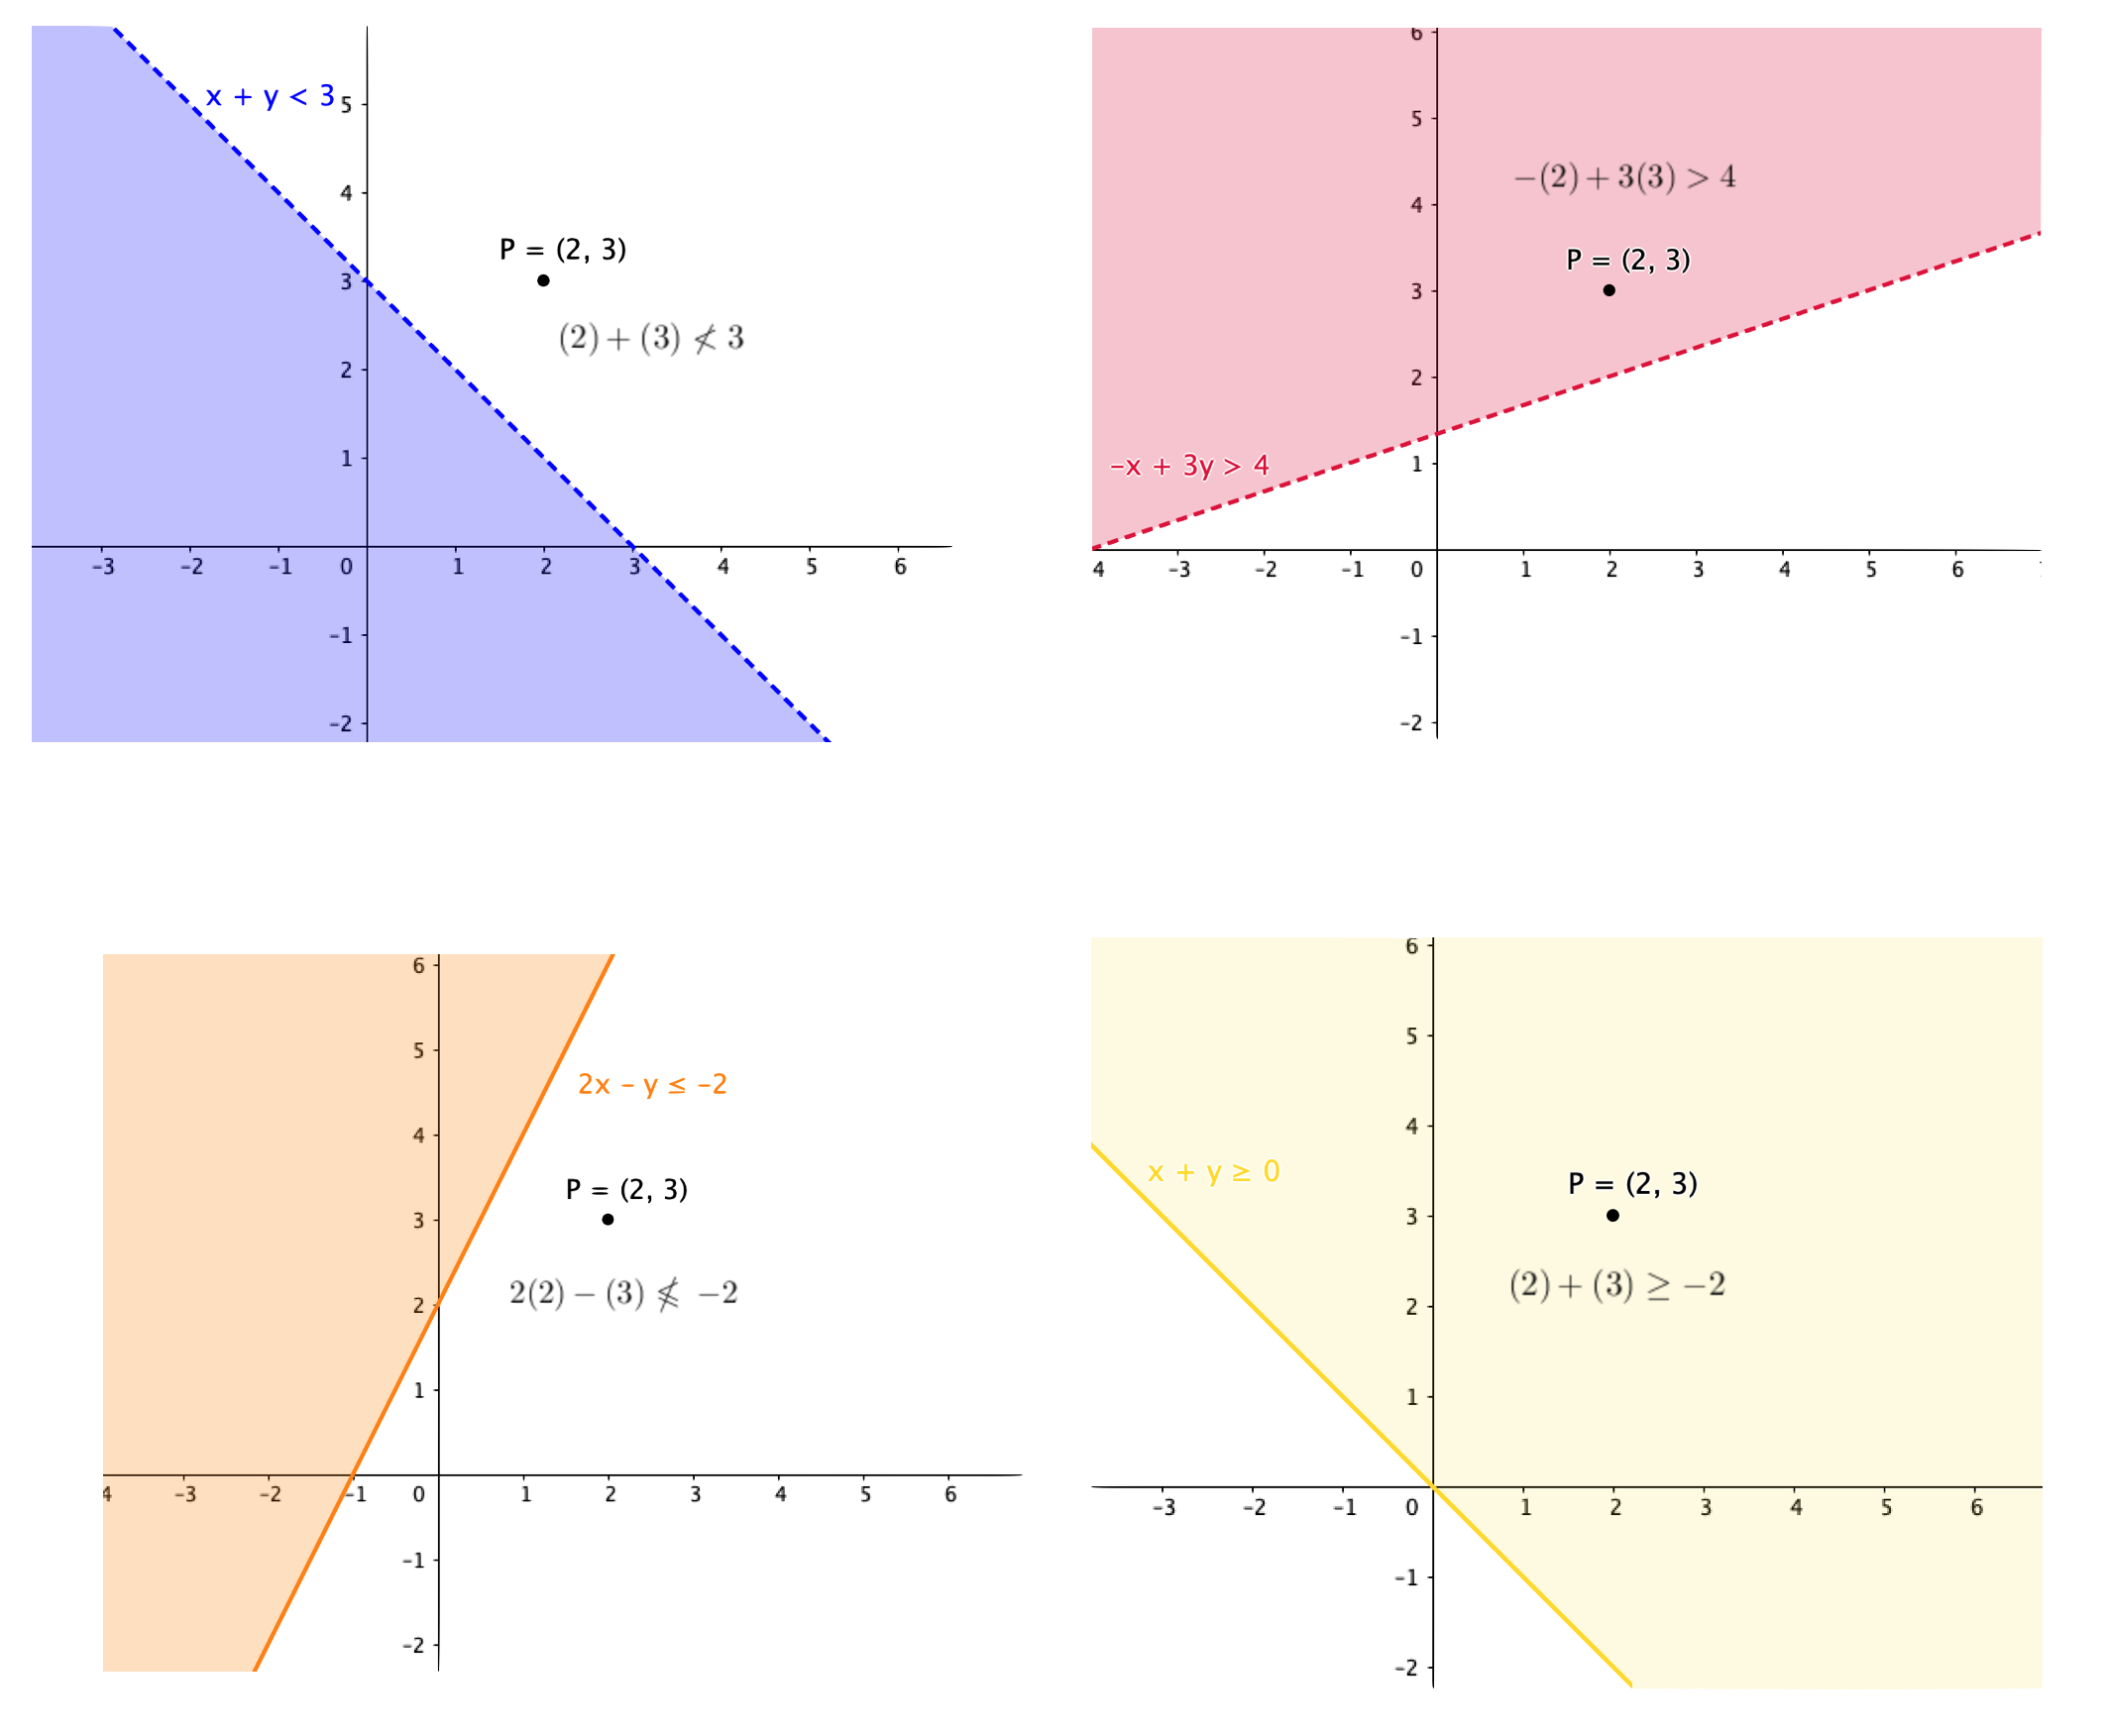
\includegraphics[width=1\textwidth]{imagenes/img07.png}
\end{figure}
\end{miejemplo}

\vspace{5mm}

\begin{theorem}
.	Un \textbf{sistema de inecuaciones lineales con dos incógnitas}	 son dos o más de estas inecuaciones que se deben verificar simultáneamente.

\vspace{5mm}
\begin{destacado}

Procedimiento para la resolución de un sistema de inecuaciones lineales con dos incógnitas:

\vspace{4mm} $\triangleright\ $ Se resuelve cada inecuación por separado, es decir, para cada una de ellas dibujamos la recta y decidimos con que semiplano nos quedamos. (podemos usar flechas para señalarlo)\footnote{Como muestra el ejemplo siguiente.}

\vspace{4mm} $\triangleright\ $ La solución del sistema, también llamada \textbf{región factible}, está formada por la zona \textbf{común} de todas las inecuaciones.

$\ $	
\end{destacado}
\end{theorem}

\vspace{5mm}
\begin{miejemplo}
. 	Resolver: $\qquad \begin{cases}
\ 2x-y\ge -4 \\ \ x+2y>4 \\ \ x+y \le 5	
\end{cases}	$

\vspace{3mm}
\rule{150pt}{0.1pt}
\vspace{3mm}

Dibujadas las tres rectas, analizamos una a una sus soluciones:

\vspace{2mm} $2x-y\ge -4$, Observamos que el punto $P(0,0)$, al sustituirlo en la inecuación, proporciona el valor $0>-4$, por lo que sí verifica esta inecuación. Deseamos quedarnos con el semiplano de la recta $2x-y=-4$ en que está $P$ y lo indicamos mediante dos flechas \textcolor{teal}{verdes}.

\vspace{2mm} Para la inecuación \textcolor{red}{$x+2y>4$}, dibujamos de modo discontinuo la recta (ya que la desigualdad no es estricta). Comprobamos que $P$ no verifica la inecuación ($0 \ngtr 4$) por lo que nos quedamos con la zona del plano en que no está $P$ y lo indicamos con flechas \textcolor{red}{rojas}.

\vspace{2mm} La última inecuación, \textcolor{blue}{$x+y\le 5$}, $P$ sí verifica la inecuación, $0<5$, por lo que indicamos esta zona con flechas \textcolor{blue}{azul} en la recta correspondiente.

\vspace{4mm} Finalmente, la zona que verifica las tres inecuaciones simultáneamente (por debajo de las rectas verde y azul y por arriba de la roja) es la destacada en la figura siguiente, es la \textbf{región factible}, en este caso  \emph{acotada}.



\begin{figure}[H]
	\centering
	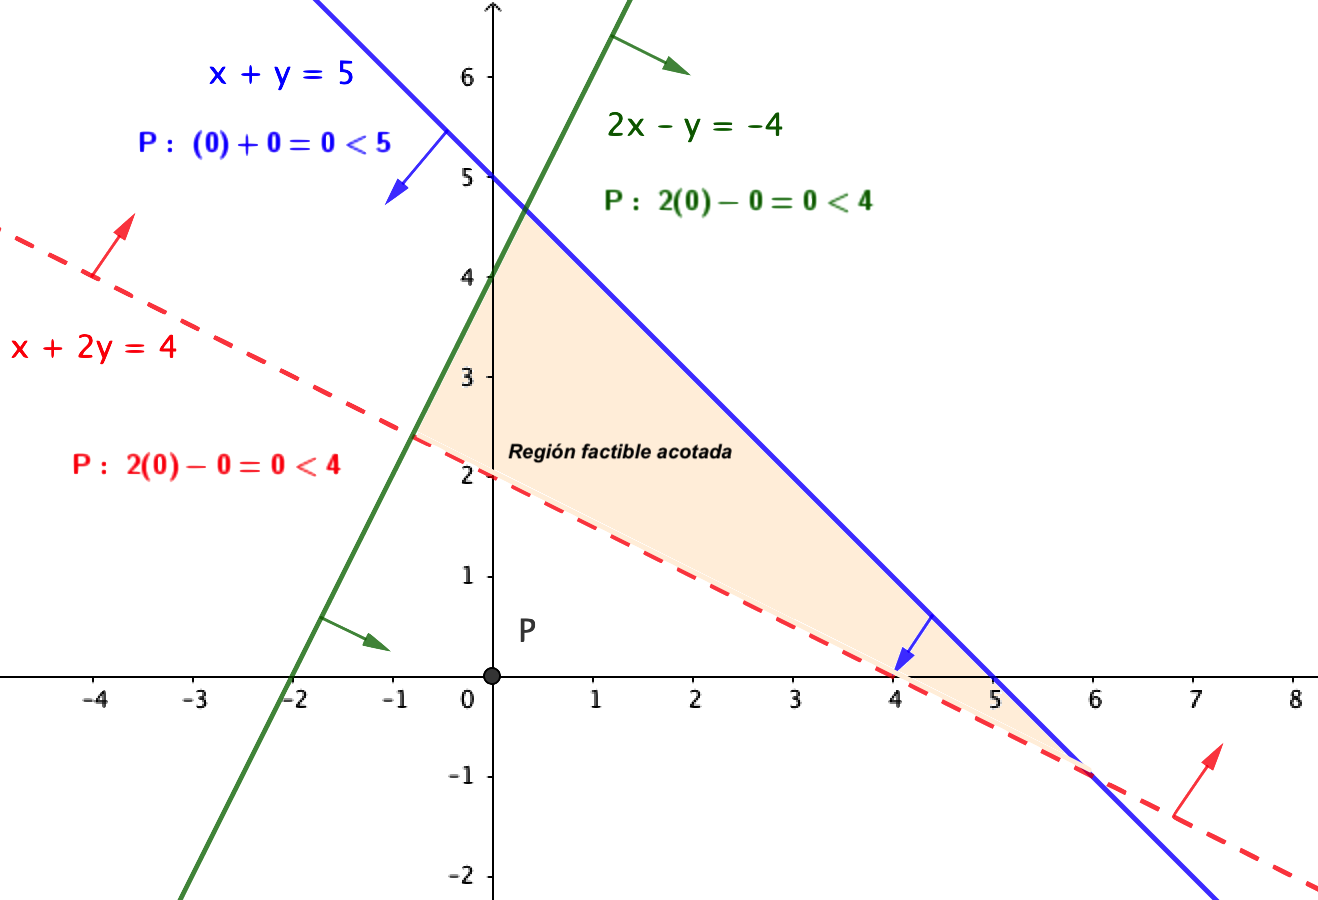
\includegraphics[width=.8\textwidth]{imagenes/img08.png}
\end{figure}

%\vspace{5mm}%**************************
Observaciones:

--- $P$ no tiene por qué ser el mismo punto para todas las inecuaciones, se puede elegir un punto prueba para cada recta.

--- \textbf{Las regiones factibles pueden ser acotadas, no acotadas o vacías}, como veremos en el siguiente ejercicio.
\end{miejemplo}

\vspace{5mm}
\begin{destacado}
$\bigstar \ $ Antes de representar las rectas correspondientes a cada inecuación es conveniente tener las tablas de valores de todas ellas para poder elegir adecuadamente la escala. 

$\bigstar \ $ Es muy conveniente poner el nombre al lado de cada recta, pronto querremos encontrar las coordenadas de los vértices del recinto factible y son las soluciones de las rectas que los forman.

$\bigstar \ $ Se recomienda hacer el gráfico	lo suficientemente grande para poder discernir si dos rectas son o no paralelas.
\end{destacado}


\vspace{5mm}
\begin{miejercicio}

Resuelve: $\quad a) \ \begin{cases}
 \ x+2y\ge 6\\ \ 2x-y\le 3	\\ \ x\ge 1
 \end{cases} \qquad
 b) \ \begin{cases}
  \ x+2y\le 6\\ \ 2x-y\le 3	\\ \ x\ge 3
 \end{cases}$


%\vspace{3mm}
\rule{150pt}{0.1pt}
\vspace{3mm}




\begin{figure}[H]
	\centering
	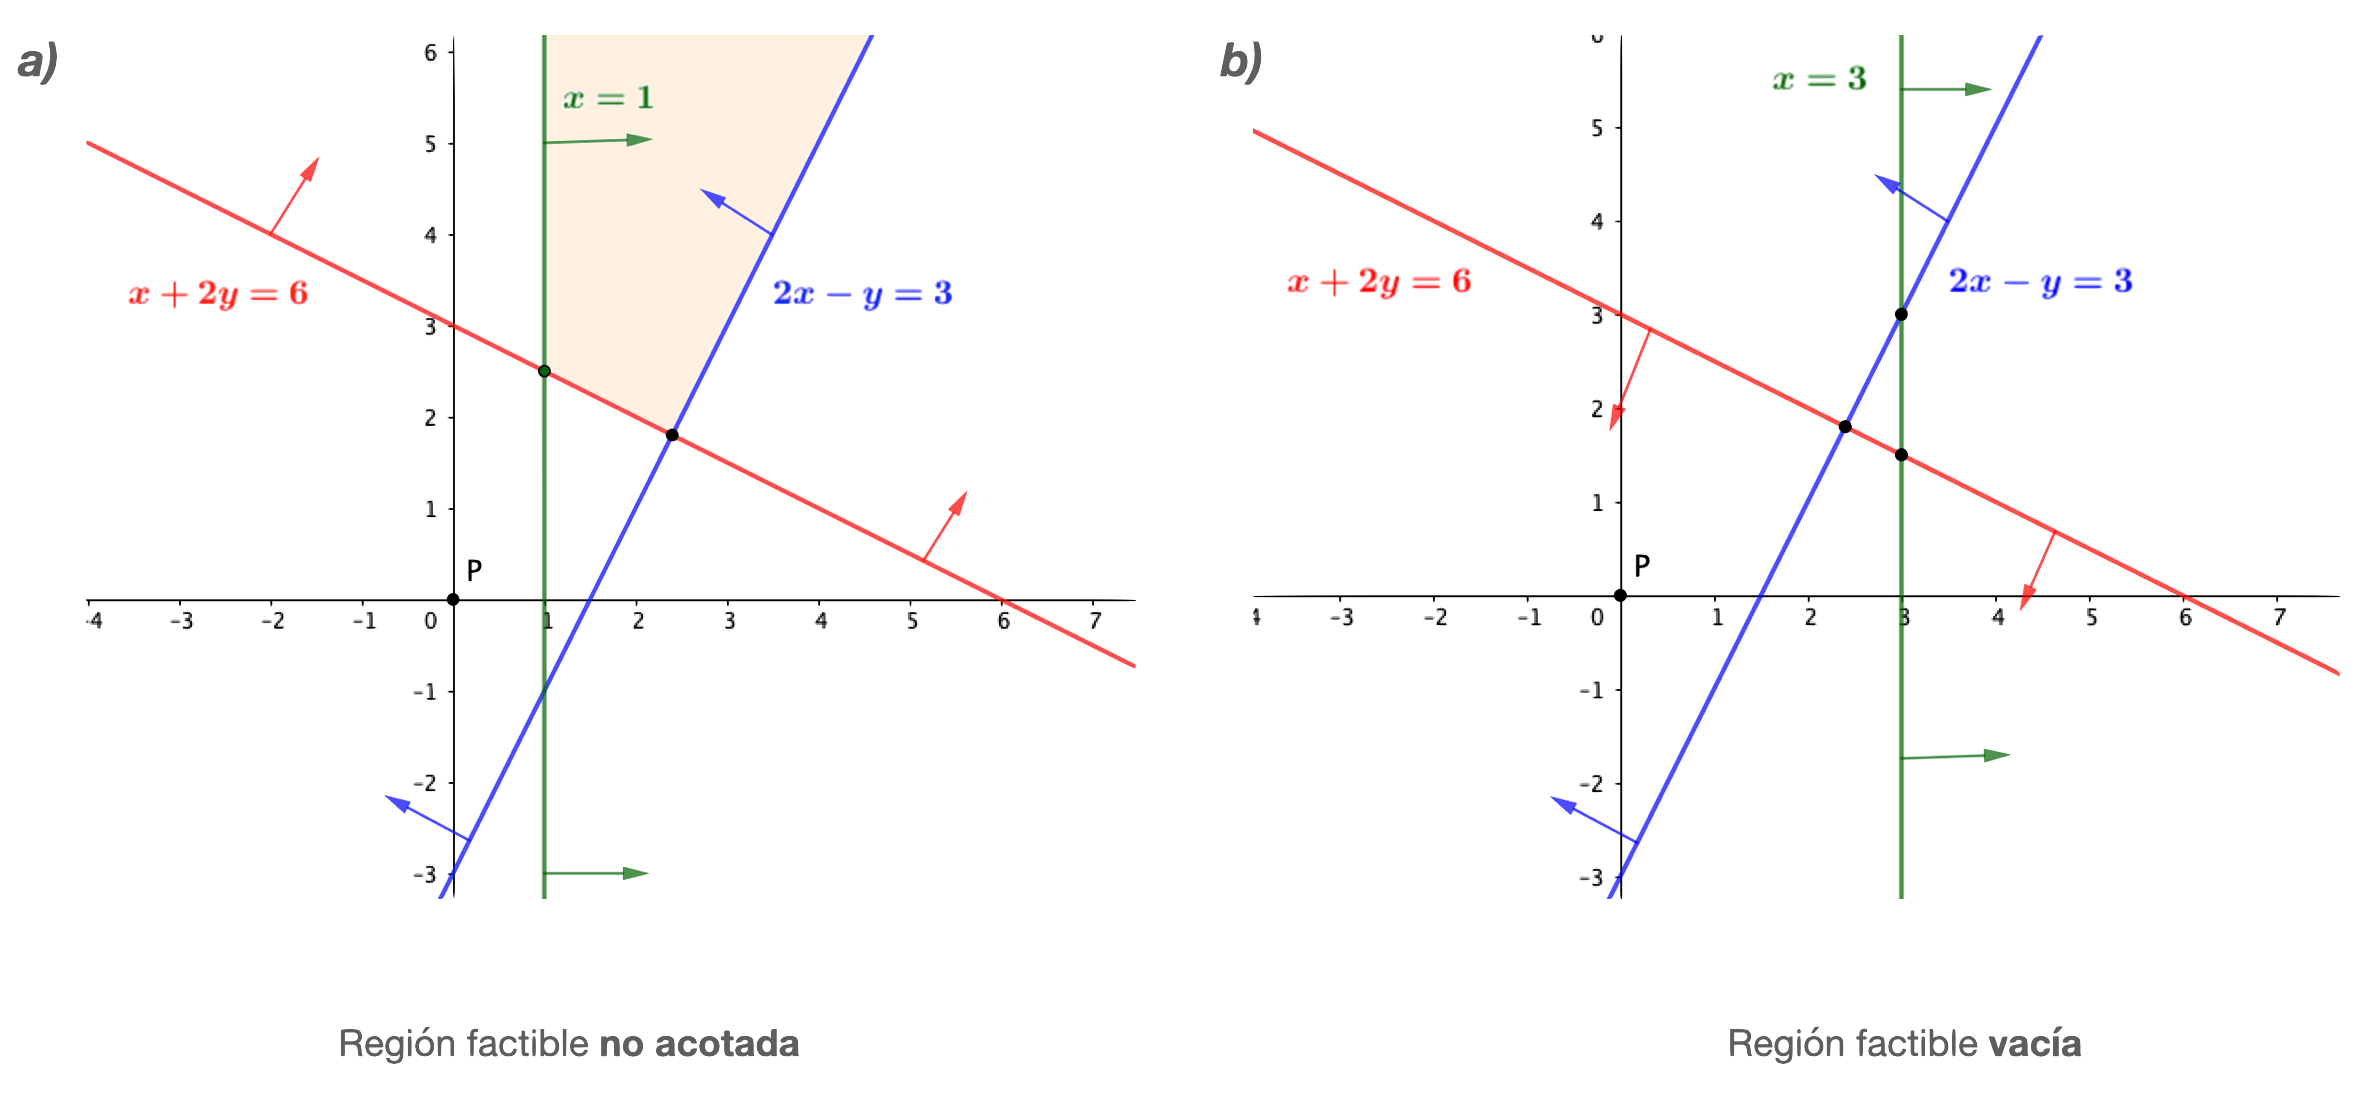
\includegraphics[width=1\textwidth]{imagenes/img09.png}
\end{figure}
\end{miejercicio}


\vspace{5mm}
\begin{miejercicio}

Para el siguiente recinto, determina las inecuaciones que lo conforman.


	\begin{figure}[H]
	\centering
	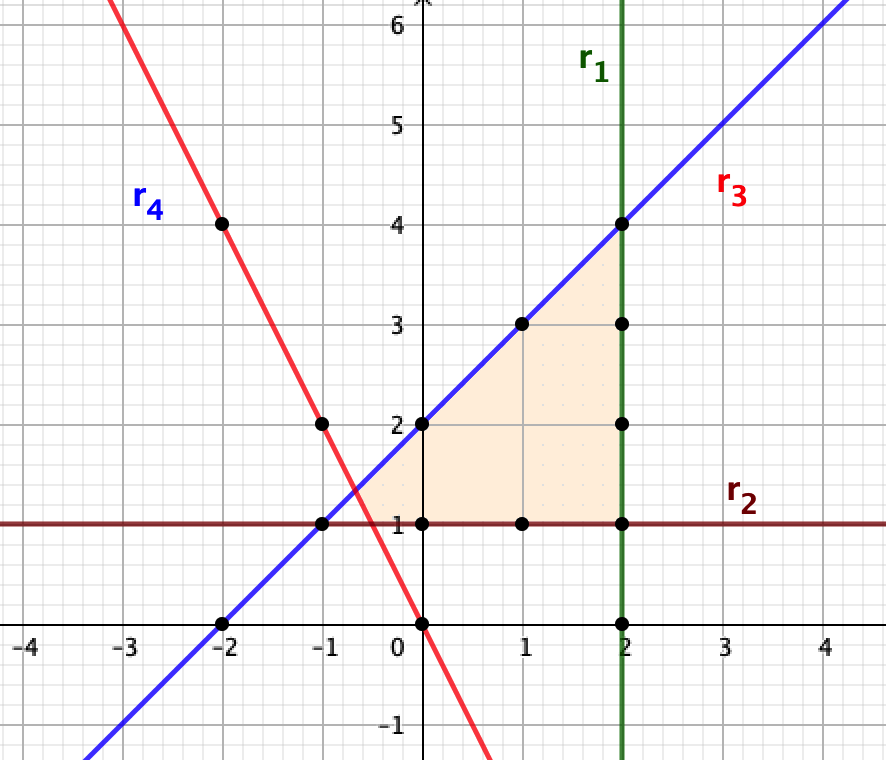
\includegraphics[width=.65\textwidth]{imagenes/img10.png}
\end{figure}

\rule{250pt}{0.1pt}

\vspace{4mm} Encontramos la ecuación de cada recta y, luego, decidiremos las zona que nos conviene.

\vspace{7mm}
--- $r_1$ es la recta vertical $x=2$, como queremos situarnos a su izquierda, la inecuación será $\boldsymbol{x\le 2}$. \textcolor{gris}{También podríamos haber decidir la zona tomando como punto prueba el origen $(0,0) \notin r_1$ y comprobar que sustituido en $r_1$, $0\le 2$, por lo que nos quedaríamos también con la zona izquierda de $x=2,\ \ x\le 2$.}



--- $r_2$ es la recta horizontal $y=1$, el semiplano superior será $\boldsymbol{y\ge 1}$.

\vspace{2mm} --- Para determinar la recta $r_3$, tomaremos dos puntos del plano por donde pase. Hemos destacado varios puntos claros en el gráfico, para $r_3$ tomamos los puntos $R_{3a}\ (-2.0)$ y  $R_{3b}\ (2,4)$. La pendiente de la recta es $m=	\dfrac{4-0}{2-(-2)}=1$, \textcolor{gris}{(si se observa claramente que la abcisa en el origen es $2$, se puede concluir que la recta es $r_3:\ y=x+2$)}. La recta es de la forma $y=1\cdot x + k$, o bien, $y-x=k$. Determinamos $k$ exigiendo que pase por uno de los puntos anteriores, p.e., si exigimos que $(2,4)\in r_3:\ y-x=k \ \to \ (4)-(2)=k \ \rightarrow \ k=2$. La recta es $r_3:\ y-x=2$

Tomando como punto prueba el origen de coordenadas: $\ 0-0=0<2$, luego queremos los puntos que hagan $\boldsymbol{y-x\le 2}$ (el trazado de la recta es continuo).

También hubiésemos podido encontrar la recta $r_3:\ y=m\cdot x+n$ exigiendo que pase por $R_{3a}$ y $R_{3b}$ y resolviendo el sistema de dos ecuaciones lineales con dos incógnitas. Las soluciones hubiesen sido $m=1, \ n=2$

La inecuación $y-x\le 2$ se pude presentar en varias formas, $y\le x+2;\ \ y-x-2\le 0,\ \ x-y+2\ge 0,\ etc$ 

\vspace{2mm} --- Finalmente, $r_4$ es una función lineal, pasa por el origen, como también pasa por $R_4\ (-2,0)$, su pendiente es $m=\dfrac{4 \textcolor{gris}{-0}}{-2 \textcolor{gris}{-0}} =-2$, por lo que $r_4:\ y=-2x$ o $y+2x=0$

Para decidir con que zona nos quedamos, al pasar $r_4$ por el origen, éste no es válido como punto prueba, hemos de tomar otro punto (que no pertenezca a $r_4$, por ejemplo el punto $(1,1)$. Como, sustituido en $r_4$ tenemos $(1)+2(1)=3>0$, tomamos como inecuación $\ \boldsymbol{y+2x\ge 0}$

\vspace{4mm} El sistema de inecuaciones que da lugar a este recinto es:
$\quad \begin{cases}
\ x\le 2 \\ \ y\ge 1 \\ \ y-x\le 2 \\ \ y+2x\ge 0$$	
\end{cases}$


\end{miejercicio}


\begin{miejercicio}

Una tienda de ropa A paga a sus empleados 1\euro $\, $ por artículo vendido más una cantidad fija de 500 \euro $\, $ al mes. Otra tienda B para 1.5 \euro $\, $ por artículo y 300 \euro $\, $ fijos al mes. ?`Cuántos atrículos ha de vender un empleado de B para ganar más dinero que uno de A?

\rule{250pt}{0.1pt}

\vspace{4mm} $x+500<1.5+300 \ \to \ 200<0.5x \ \to 400<x\, . \ $ Ha de vender más de 400 artículos al mes.
	
\end{miejercicio}

\begin{miejercicio}

En una reunión tres personas, Ana, Belen y César, hablan de sus edades. Sabemos que entre los tres tienen 85 años, que Belen tiene el doble de edad que Ana y que César tiene 15 años más que Belen. ?`El más joven de ellos es mayor de edad?

\rule{250pt}{0.1pt}

\vspace{4mm} Edades: x=Ana, y=Belen, z=César. 

\vspace{2mm}$\begin{cases}\ x+y+z<85 \\ \ y=2x\\ \ z=15+y=15+2x \end{cases} \ \to \ x+2x+15+2x<85 \ \to \ 5x<70 \ \to \ x<14$

\vspace{2mm} Ana, la más joven, tiene x=14 años, es menor de edad.
	
\end{miejercicio}

\begin{miejercicio}

Un gimnasio cobra a sus socios una cuota mensual de 36 euros, lo que les da derecho a disfrutar de las instalaciones tantas horas al mes como deseen. Una persona que no sea socia tiene que pagar 4.50 euros a la hora por utilizar dicha instalaciones. ?`Cuántas horas mensuales tendrá que jugar una persona para que le salga más rentable hacerse socia del club?

\rule{250pt}{0.1pt}

\vspace{4mm} $36<4.5 x \ \to \ x>8\, . \ $ Ha de usar las instalaciones más de 8h al mes.

\end{miejercicio}

\begin{myalertblock}{Inecuaciones de segundo grado con dos incógnitas}

\vspace{5mm}
	$\triangleright \quad $ \textbf{Inecuaciones de la forma:} $\ \ \boldsymbol {dy+ax^2+bx+c<0}\ \ $  \begin{footnotesize}(o cualquier otra desigualdad)\end{footnotesize}
	
\vspace{2mm} Despejando $\ \ y<Ax^2+Bx+C\ \ $ \textcolor{gris}{con $A=-a/d;\ B=-b/d;\ C=-c/d$ }

\vspace{2mm} $y=Ax^2+Bx+C$ es una \textbf{parábola} que divide el plano en dos semiplanos, en uno de ellos se verificará que $y>Ax^2+Bx+C$ y en el otro $y<Ax^2+Bx+C$

\vspace{2mm} Elegido un punto cualquiera que no esté en la parábola,   verificamos si ese punto cumple o no la inecuación de partida. Si la respuesta es sí, la zona donde está el punto es el semiplano solución, si es no, se trata de la zona opuesta.	

\vspace{5mm}

\begin{figure}[H]
		\centering
		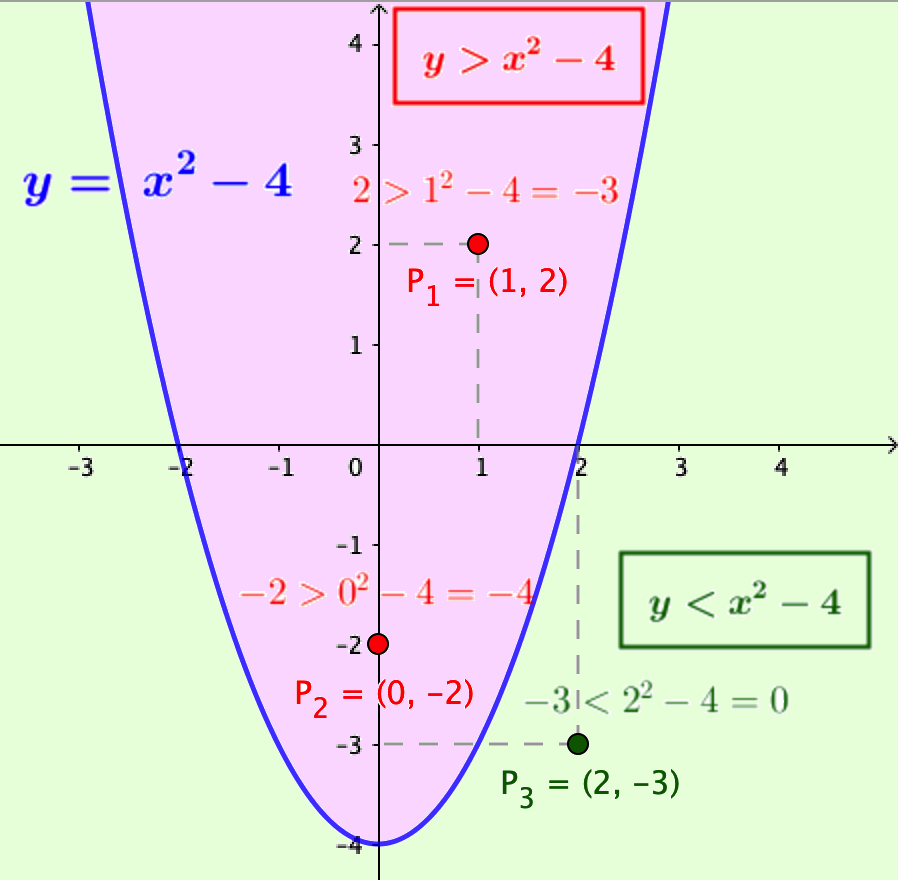
\includegraphics[width=0.55\textwidth]{img-ecc/ecc15.png}
	\end{figure}


\vspace{5mm} El el tema de cónicas estudiarás la parábola, hipérbola, elipse y circunferencia. Son casos particulares de expresiones denominadas \emph{cuádricas} que tienen la forma $\ Ax^2 + By^2 + Cxy + Dx + Ey  + F = 0 $


\end{myalertblock}



\vspace{1cm}
\section{Ejercicios}

\begin{tikzpicture}
	\fill [left color=red!50, right color=teal!50] (0,0) rectangle (3.5,.1);
	\fill [left color=teal!50, right color=blue!50] (3.5,0) rectangle (7.5,.1);
	\end{tikzpicture}
\vspace{0.5cm}


%*******
\begin{mipropuesto}
. \begin{multicols}{2}
 \begin{enumerate}[a)  ]	
 \item 	$4-3x+1\leqslant9-8x+6$
 \item $6-7x>4x+6$
 \item $(3-4x)-(5x-4)>6x-(3x-4)$
 \item $x-15\geqslant x$
 \end{enumerate}
 \end{multicols}

\end{mipropuesto}
\vspace{-8mm}
\begin{flushright}
	\begin{footnotesize} \textcolor{gris}{\rotatebox{180}{ $a)\ \ ]-\infty,2];\quad b)\ \ ]-\infty,0[;\quad c)\ \ ]-\infty,1/4[;\quad d)\ \ \nexists $ solución}}	\end{footnotesize}
\end{flushright}

%*******
\begin{mipropuesto}
. $a)\quad \dfrac{5x-1}{25}-\dfrac{4x+1}{5} \leqslant \dfrac{2x-7}{5}-x\, ; \qquad \qquad b) \quad \dfrac{7x+1}{2} > \dfrac{5}{6}x+\dfrac{8x}{3}$
\end{mipropuesto}
\vspace{-8mm}
\begin{flushright}
	\begin{footnotesize} \textcolor{gris}{\rotatebox{180}{ $a)\ \ \nexists $ solución $\quad b)\ \ \mathbb R$ }}	\end{footnotesize}
\end{flushright}

%*******
\begin{mipropuesto}
. $ a)\quad \begin{cases} \ 5x-4\geqslant 2x+2 \\ \ 3x-8 \leqslant x+6 \end{cases} \qquad \qquad  
b)\quad \begin{cases} \ 10x<8  \\ \ 1+3x>2x+4 \end{cases} $
\end{mipropuesto}
\vspace{-8mm}
\begin{flushright}
	\begin{footnotesize} \textcolor{gris}{\rotatebox{180}{ $a)\ \ [2,7]; \qquad b)\ \ \nexists $ solución}}	\end{footnotesize}
\end{flushright}

%*******
\begin{mipropuesto}
. Determinar el valor de $m$ para que $\ 3x-m<1\ $ tenga por solución $\ ]-\infty, 5[$
\end{mipropuesto}
\vspace{-8mm}
\begin{flushright}
	\begin{footnotesize} \textcolor{gris}{\rotatebox{180}{ Resuleve en función de $m$ e identifica con el resultado esperado, $\ m=-14$ }}	\end{footnotesize}
\end{flushright}

%*******
\begin{mipropuesto}
. $a)\ \ 3-8x+3x^2>2x^2-6x+3\, ; \qquad \qquad b)\ \ x(x-1)\leqslant 2x-9$
\end{mipropuesto}
\vspace{-8mm}
\begin{flushright}
	\begin{footnotesize} \textcolor{gris}{\rotatebox{180}{ $a)\ \ ]-\infty, 0[ \ \cup \ ]2,+\infty[;\qquad b)\ \ [-1,9]$}}	\end{footnotesize}
\end{flushright}

%*******
\begin{mipropuesto}
. $a)\ \ \begin{cases} \ x^2-7x+6<0 \\ \ x^2-10x+16 < 0 \end{cases} \qquad \qquad b)\ \ \begin{cases} \ x^2-8x+15<0 \\ \ 3x+1\geqslant x+9 \end{cases}$
\end{mipropuesto}
\vspace{-8mm}
\begin{flushright}
	\begin{footnotesize} \textcolor{gris}{\rotatebox{180}{ $a)\ \ ]2,6[\, ; \qquad b)\ \ [4,5[$ }}	\end{footnotesize}
\end{flushright}


%*******
\begin{mipropuesto}
. $a)\ \ \dfrac{7}{2x-1}<3 \, ; \qquad \qquad b)\ \ \dfrac{x-1}{x+3} < 1 \, ; \qquad \qquad c)\ \ \dfrac{1}{x+1}\leqslant 1+\dfrac{2}{x-1}$
\end{mipropuesto}
\vspace{-8mm}
\begin{flushright}
	\begin{footnotesize} \textcolor{gris}{\rotatebox{180}{ $a)\ \ ]-\infty, 1/2[ \ \cup \ ]5/3,+\infty[\, ; \qquad b)\ \ ]-\infty,+\infty[ \equiv \mathbb R \, ; \qquad c)\ \ ]-\infty,-1[ \ \cup \ ]1,+\infty[$ }}	\end{footnotesize}
\end{flushright}

%*******
\begin{mipropuesto}
. $a)\ \ x^3-5x^2+2x+8\geqslant 0;\qquad b)\ \dfrac{x^2-2}{x}<\dfrac{x^2+4x-2}{x^2+x}; \qquad c)\ \dfrac{x}{4x-x^2}\geqslant 1$
\end{mipropuesto}
\vspace{-8mm}
\begin{flushright}
	\begin{footnotesize} \textcolor{gris}{\rotatebox{180}{ $a)\ \ [-1,2]\, \cup\, [4,+\infty[;\qquad b)\ ]-\infty,-\sqrt{6}[\, \cup \, ]\sqrt{6},+\infty[;\qquad c)\ [3,4[$ }}	\end{footnotesize}
\end{flushright}

%*******
	\begin{mipropuesto}
	. $a)\ \ \sqrt{x}\leqslant \dfrac 1 3 ;\qquad b)\ \ \sqrt{x+2}>2;\qquad c)\ \ \dfrac{-1}{\sqrt{2x+3}}>-2$
	\end{mipropuesto}
	\vspace{-8mm}
	\begin{flushright}
		\begin{footnotesize} \textcolor{gris}{\rotatebox{180}{ $a)\ [0,1/9];\qquad b)\ [2,+\infty[;\qquad c)\ ]-11/8,+\infty[$}}	\end{footnotesize}
	\end{flushright}

%*******
\begin{mipropuesto}
. $ a) \ \begin{cases} \ \dfrac{3-x}{3}-2 < \dfrac{4-2x}{2}  \\  \ \dfrac{2-x}{5} \leqslant 3-x \end{cases} \qquad b)\  \begin{cases} \ 2-\dfrac{3+5x}{4}>x \\ \ x^2-3x-10\leqslant 0 \end{cases} \qquad c)\ \ \begin{cases} \ x^2-x-1<0 \\ \ x^2+4\leqslant (x+2)^2 \\ x+7>3x+5 \end{cases}$
\end{mipropuesto}
\vspace{-8mm}
\begin{flushright}
	\begin{footnotesize} \textcolor{gris}{\rotatebox{180}{ $a)\ \ ]-\infty,13/4];\qquad b)\ \ [-2,5/9[; \qquad c)\ \ [0,1[$ }}	\end{footnotesize}
\end{flushright}

%*******
\begin{mipropuesto}
. $a)\ \ \left| 1-\dfrac x 3 \right| < 1 ;\qquad  b)\ \ \left| \dfrac{2x-1}{1+2x} \right| > 3; \qquad c)\ \ |2x+5|\geqslant |x+4|;\qquad d)\ \ \left| \dfrac{x-3}{5x} \right| < \dfrac 1 3  $
\end{mipropuesto}
\vspace{-8mm}
\begin{flushright}
	\begin{footnotesize} \textcolor{gris}{\rotatebox{180}{ $a)\ ]0,6[;\qquad b)\ ]-1,-1/2[\, \cup ]-1/2,-1/4[ ; \qquad c)\ ]-\infty,-3]\, \cup \, [-1,+\infty[;\qquad d)\ ]-\infty, -9/2[\, \cup \, ]9/8,+\infty[ $ }}	\end{footnotesize}
\end{flushright}

%*******
\begin{mipropuesto}
. $a)\ \begin{cases} 
 \ |x+6|>5 \\ \ |x-8|<20	
 \end{cases} \qquad \qquad \qquad b)\ \begin{cases}
 \ |2x-1|\geqslant 3 \\ \ x^2+5>6x	
 \end{cases}$

\end{mipropuesto}
\vspace{-8mm}
\begin{flushright}
	\begin{footnotesize} \textcolor{gris}{\rotatebox{180}{ $a)\ \ ]-12,-11[ \, \cup \, ]-1,28[;\qquad b)\ \ ]-\infty,-1] \, \cup \, ]5,+\infty[$ }}	\end{footnotesize}
\end{flushright}


	


%%%%%%%%%%%%%%%%%%%%%%%%%%%%%%%%%%%%%%%%%%%%%%%%%

\newpage

$\qquad$


\begin{adjustwidth}{50pt}{250pt}
\begin{cuadro-naranja}
\textbf{\huge{Problemas $\boldsymbol{+}$}}\normalsize{$\, $}
\end{cuadro-naranja}	
\end{adjustwidth}



\vspace{5mm}
\begin{enumerate}[\textbf{P$\boldsymbol +$} 1. ]
\item	 Determina los valores de $m$ y $n$ para que $\ mx^2+7x+n>0\ $ tenga por solución $\ ]2,5[$

\vspace{-6mm}
\begin{flushright}
\begin{footnotesize} \textcolor{gris}{\rotatebox{180}{ 2 y 5 han de ser soluciones de la ecuación de segundo grado $\ \to \ m=-1,\ n=-10\, . \ \  $ Compruébalo.  }}	\end{footnotesize}
\end{flushright}

%%%%
\item	Hace 10 años la edad de Xavier era inferior a la mitad de su edad actual y dentro de 10 años no superará al doble de la edad que tiene ahora. ?`Cual es la edad de Xavier?

\vspace{-6mm}
\begin{flushright}
\begin{footnotesize} \textcolor{gris}{\rotatebox{180}{ La edad ha de ser natural, Xavier tiene 19 años. }}	\end{footnotesize}
\end{flushright}


%%%%
\item	$|x-1| \leqslant 2|x-3|$

\vspace{-6mm}
\begin{flushright}
\begin{footnotesize} \textcolor{gris}{\rotatebox{180}{ Llegarás a $\ 3x^2-22x+35 \geqslant 35 \ \to \ \ sol:\ \ [7/3,5]$ }}	\end{footnotesize}
\end{flushright}

\vspace{-12mm}
\begin{flushright}
\begin{tiny} \textcolor{gris}{\rotatebox{180}{ \textbf{Para probar una desigualdad entre 2 números positivos es suficiente con probar esa desigualdad para sus cuadrados. }}}	\end{tiny}
\end{flushright}

%%%%
\item	$\left| \dfrac{x+2}{x-6} \right| - \left| \dfrac{x-1}{x-3} \right| \ \leqslant \ 0$

\vspace{-6mm}
\begin{flushright}
\begin{scriptsize} \textcolor{gris}{\rotatebox{180}{ Con la misma estratégia que en el caso anterior, llegará a $ \ 12x^3-72x^2+96\leqslant 0 \ \to \ sol: \ ]-\infty,0]\,\cup\, [2,4] \smallsetminus  \{3\}$ }}	\end{scriptsize}
\end{flushright}

%%%%
\item	$\sqrt{1+mx} \ = \ x \ + \ \sqrt{1-mx}$

\vspace{-10mm}
\begin{flushright}
\begin{scriptsize} \textcolor{gris}{\rotatebox{180}{ Aisla las raíces en un miembro y multiplica y divide por su conjugado. $\quad x=0 \ \wedge \ x=\pm\sqrt{1-m^2} ;\ \ \  m\in [1/\sqrt{2} ,\, 1]$ }}	\end{scriptsize}
\end{flushright}


%%%%
\item	En una granja, hay, al menos, 28 animales entre gallinas y conejos.

El número de conejos es superior al doble de la diferencia entre el número de gallinas y 12, y el número de gallinas es superior a 9 veces la diferencia entre el número de conejos y 10.

?`Cuál es la diferencia entre el número de gallinas y el de conejos?


\vspace{-8mm}
\begin{flushright}
\begin{scriptsize} \textcolor{gris}{\rotatebox{180}{ Solución, 17 gallinas y 11 conejos, la diferencia entre ellos es 6. }}	\end{scriptsize}
\end{flushright}

\vspace{-12mm}
\begin{flushright}
\begin{scriptsize} \textcolor{gris}{\rotatebox{180}{  Luego, cuando resuelvas (por reducción) impón la condición sobre el número total de animales. }}	\end{scriptsize}
\end{flushright}

\vspace{-12mm}
\begin{flushright}
\begin{scriptsize} \textcolor{gris}{\rotatebox{180}{ Escribe un sistema de inecuaciones con las condiciones del número de animales de cada clase.  }}	\end{scriptsize}
\end{flushright}


%%%%
\item	Resuelve $ \quad 2^{4^x}\ <\ 4^{2^x}$

\vspace{-10mm}
\begin{flushright}
\begin{scriptsize} \textcolor{gris}{\rotatebox{180}{ Escribe todo como potencias de base 2. $\quad \text{sol: } \ ]-\infty, 1[$ }}	\end{scriptsize}
\end{flushright}

\end{enumerate}


%%%%%%%%%%%%%%%%%%%%%%%%%%%%%%%%%%%%%%%

\vspace{1cm}
\section{Resumen del tema}

\begin{tikzpicture}
	\fill [left color=red!50, right color=teal!50] (0,0) rectangle (3.5,.1);
	\fill [left color=teal!50, right color=blue!50] (3.5,0) rectangle (7.5,.1);
	\end{tikzpicture}
\vspace{0.5cm}

\begin{myblock}{Resumen  \emph{``Inecuaciones''}}

\vspace{2mm} \emph{Al multiplicar (dividir) una inecuación por una cantidad negativa, el sentido de ésta cambia. $\ (*)$}

\vspace{2mm} $\triangleright \quad $ \textbf{inecuación lineal con 1 incógnita} $\ \to \ $ despejar $\ \ (*)$

\vspace{2mm}  $\triangleright \quad $ \textbf{inecuación con 1 incógnita} $\ \to \ $ estudios signos (tabla).

\vspace{2mm}  $\triangleright \quad $ \textbf{sistema de inecuaciones con 1 incógnita} $\ \to \ $ intersección de las soluciones de cada una de las inecuaciones que lo conforman.

\vspace{2mm}  $\triangleright \quad $ \textbf{inecuación lineal con 2 incógnita} $\ \to \ $ semiplanos.

\vspace{2mm}	
\end{myblock}





\begin{comment}

%%%%%%%%%%%%%%%%%%%%%%%%%%%%%%%%%%%. SECCIONES

\begin{figure}[H]
	\centering
	
\includegraphics[width=0.35\textwidth]{img-pol/pol05.png}
\end{figure}


\chapter{texto}

\begin{tikzpicture}
	\fill [left color=red!50, right color=teal!50] (0,0) rectangle (6.5,.2);
	\fill [left color=teal!50, right color=blue!50] (6.5,0) rectangle (11.5,.2);
	\end{tikzpicture}

\vspace{1cm}
\section{texto}

\begin{tikzpicture}
	\fill [left color=red!50, right color=teal!50] (0,0) rectangle (3.5,.1);
	\fill [left color=teal!50, right color=blue!50] (3.5,0) rectangle (7.5,.1);
	\end{tikzpicture}
\vspace{0.5cm}

\subsection{texto}
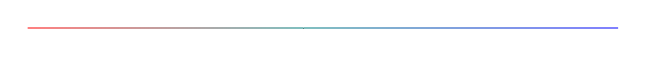
\begin{tikzpicture}
	\fill [left color=red!50, right color=teal!50] (0,0) rectangle (3.5,.01);
	\fill [left color=teal!50, right color=blue!50] (3.5,0) rectangle (7.5,.01);
	\end{tikzpicture}
\vspace{0.5cm}


%%%%%%%%%%%%%%%%%%%%%%%%%%%%%%%%%%%. \begin{ ------>. 
detsacado;  cuadro-naranja;  cuadro-gris;  miejercicio (solución extensa);  mipropuesto (solución corta y fuera del cuadro)

%%%%%%%%%%%%%%%%%%%%%%%%%%%%%%%%%%%. CURIOSIDAD
\vspace{1cm}
\color{ForestGreen!80}
\rule{250pt}{0.2pt}
Texto
\vspace{-8mm}
\begin{flushright}
\rule{250pt}{0.2pt}		
\end{flushright}	
\color{black}
\end{comment}